\documentclass[titlepage]{article}
\usepackage[spanish,es-tabla]{babel}

% Set page size and margins
% Replace `letterpaper' with `a4paper' for UK/EU standard size
\usepackage[a4paper,top=2cm,bottom=2cm,left=3cm,right=3cm,marginparwidth=1.75cm]{geometry}

% DIBUJOS
\usepackage{amsmath}
\usepackage{graphicx}
\usepackage[colorlinks=true, citecolor=blue, linkcolor=black]{hyperref}

%%TABLES
\usepackage{colortbl}
\usepackage{hhline}
\usepackage{color}
\usepackage{tabularray}
\usepackage[table,xcdraw]{xcolor}

%%ÍNDICE
\usepackage{titlesec}
\usepackage{blindtext}

%%PSEUCODE
\usepackage[spanish, linesnumbered,ruled,vlined]{algorithm2e}

%%%CODE
\usepackage{listings}

%%BIBLIOGRAFIA
\usepackage{apacite}
\bibliographystyle{apacite}

%%INTERLINEADO DOBLE
\renewcommand{\baselinestretch}{2}

%%INTERLINEADO EN BLOQUES CONCRETOS
\usepackage{setspace}

%%FOOTNOTES
\usepackage[para, multiple]{footmisc}
\setlength{\skip\footins}{1cm}
\renewcommand{\footnotesize}{\scriptsize}

%%IN-LINE CODE
\usepackage{listings}
\usepackage{color}

%%---TIMES NEW ROMAN---
\usepackage{mathptmx} % Usa Times New Roman para texto y matemáticas 
\usepackage[utf8]{inputenc} % Manejo de caracteres UTF-8 
\usepackage[T1]{fontenc} % Codificación de fuentes


\lstset{frame=tb,
  language=Java,
  aboveskip=3mm,
  belowskip=3mm,
  showstringspaces=false,
  columns=flexible,
  basicstyle={\small\ttfamily},
  numbers=none,
  numberstyle=\tiny\color{gray},
  keywordstyle=\color{blue},
  commentstyle=\color{dkgreen},
  stringstyle=\color{mauve},
  breaklines=true,
  breakatwhitespace=true,
  tabsize=3
}

%%INFORMACIÓN
\title{¿En qué medida las técnicas de concurrencia optimizan el algoritmo de ordenación Merge Sort?}
\author{Gabriel Ruiz Díaz}
\date{}

%%% UNICODE
\usepackage[utf8]{inputenc}

%%%PGFPLOTS
\usepackage{pgfplots}
\pgfplotsset{compat=1.18}
%%%%CAPTION
\usepackage{caption}

%%%%%FIGURAS ADAPTADAS
\usepackage{wrapfig}

%%%%%Forzar figuras con H
\usepackage{float}

\begin{document}
	
\definecolor{dkgreen}{rgb}{0,0.6,0}
\definecolor{gray}{rgb}{0.5,0.5,0.5}
\definecolor{mauve}{rgb}{0.58,0,0.82}	
	
%%%%PORTADA%%%%%%%%%%%%%%%%%
\begin{titlepage}
\centering
{\hfill}
\vspace{3cm}

{\Huge El algoritmo de ordenación por mezcla\par}
\vspace{2cm}
{\LARGE ¿En qué medida las técnicas de concurrencia optimizan el algoritmo de ordenación \textit{Merge Sort}? \par}
\vspace{1cm}
{\scshape\large Monografia de Informática NS \par}
\vspace{8cm}


{\Large Cómputo de palabras: xxxx \par}
{\Large Código del alumno: lqv708 \par}
\end{titlepage}

\newpage
\tableofcontents

\newpage
%%%%%%%%%%%%%%%INTRODUCIÓN%%%%%%%%%%%%%%%%%%%%%%
%%%%%%%%%%%%%%%%%%%%%%%%%%%%%%%%%%%%%%%%%%%%%%%%
\section{Introducción}
En el día a día usamos estructuras de datos ordenadas, como la lista de contactos del teléfono, en los almacenes para la gestión de inventario, en los resultados de una búsqueda en internet, etc. El proceso de colocar los datos en un cierto orden se llama ordenación.\footnote{\cite{knuth-1997}} La ordenación es una operación común en los sistemas informáticos y ha sido ampliamente estudiada.\footnote{\cite{McMillan-2007}} Aun así, no existe un algoritmo de ordenación perfecto. Actualmente, se siguen desarrollando, y además estos relacionan una gran variedad de conceptos de informática, como la concurrencia, el paralelismo, la ejecución serial, la iteración o la recursión.
Algunos algoritmos ordenación comunes son la ordenación de burbuja, por insersción, rápido (\textit{quicksort}).
%%167 words

La finalidad de esta investigación evaluar holísticamente cuatro implementaciones del algoritmo de ordenación Merge Sort en términos de complejidad temporal y espacial, del peor caso; tiempos de ejecución y memoria usados; además de la naturaleza específica de cada implementación. Concretamente, se comparan el Merge Sort Iterativo Serial (MSIS), el Merge Sort Recursivo Serial (MSRS), el Merge Sort Recursivo Paralelo (MSRP), y el Merge Sort Iterativo Paralelo (MSIP).

%%64 words


\subsection{Merge Sort}
El ordenamiento por mezcla es un algoritmo de ordenación inspirado en la técnica divide y vencerás. Es capaz de ordenar un conjunto de datos a través de, primero, dividir la colección en dos mitades, dividir las sub-colecciones en más mitades hasta que contengan cero o un elemento, ordenar cada sub-colección, unir (\textit{merge}) todas las sub-colecciones de forma ordenada, y, finalmente la colección queda ordenada.\footnote{\cite{skiena-2008}}

%%130 words

\begin{figure}[h]
    \centering
    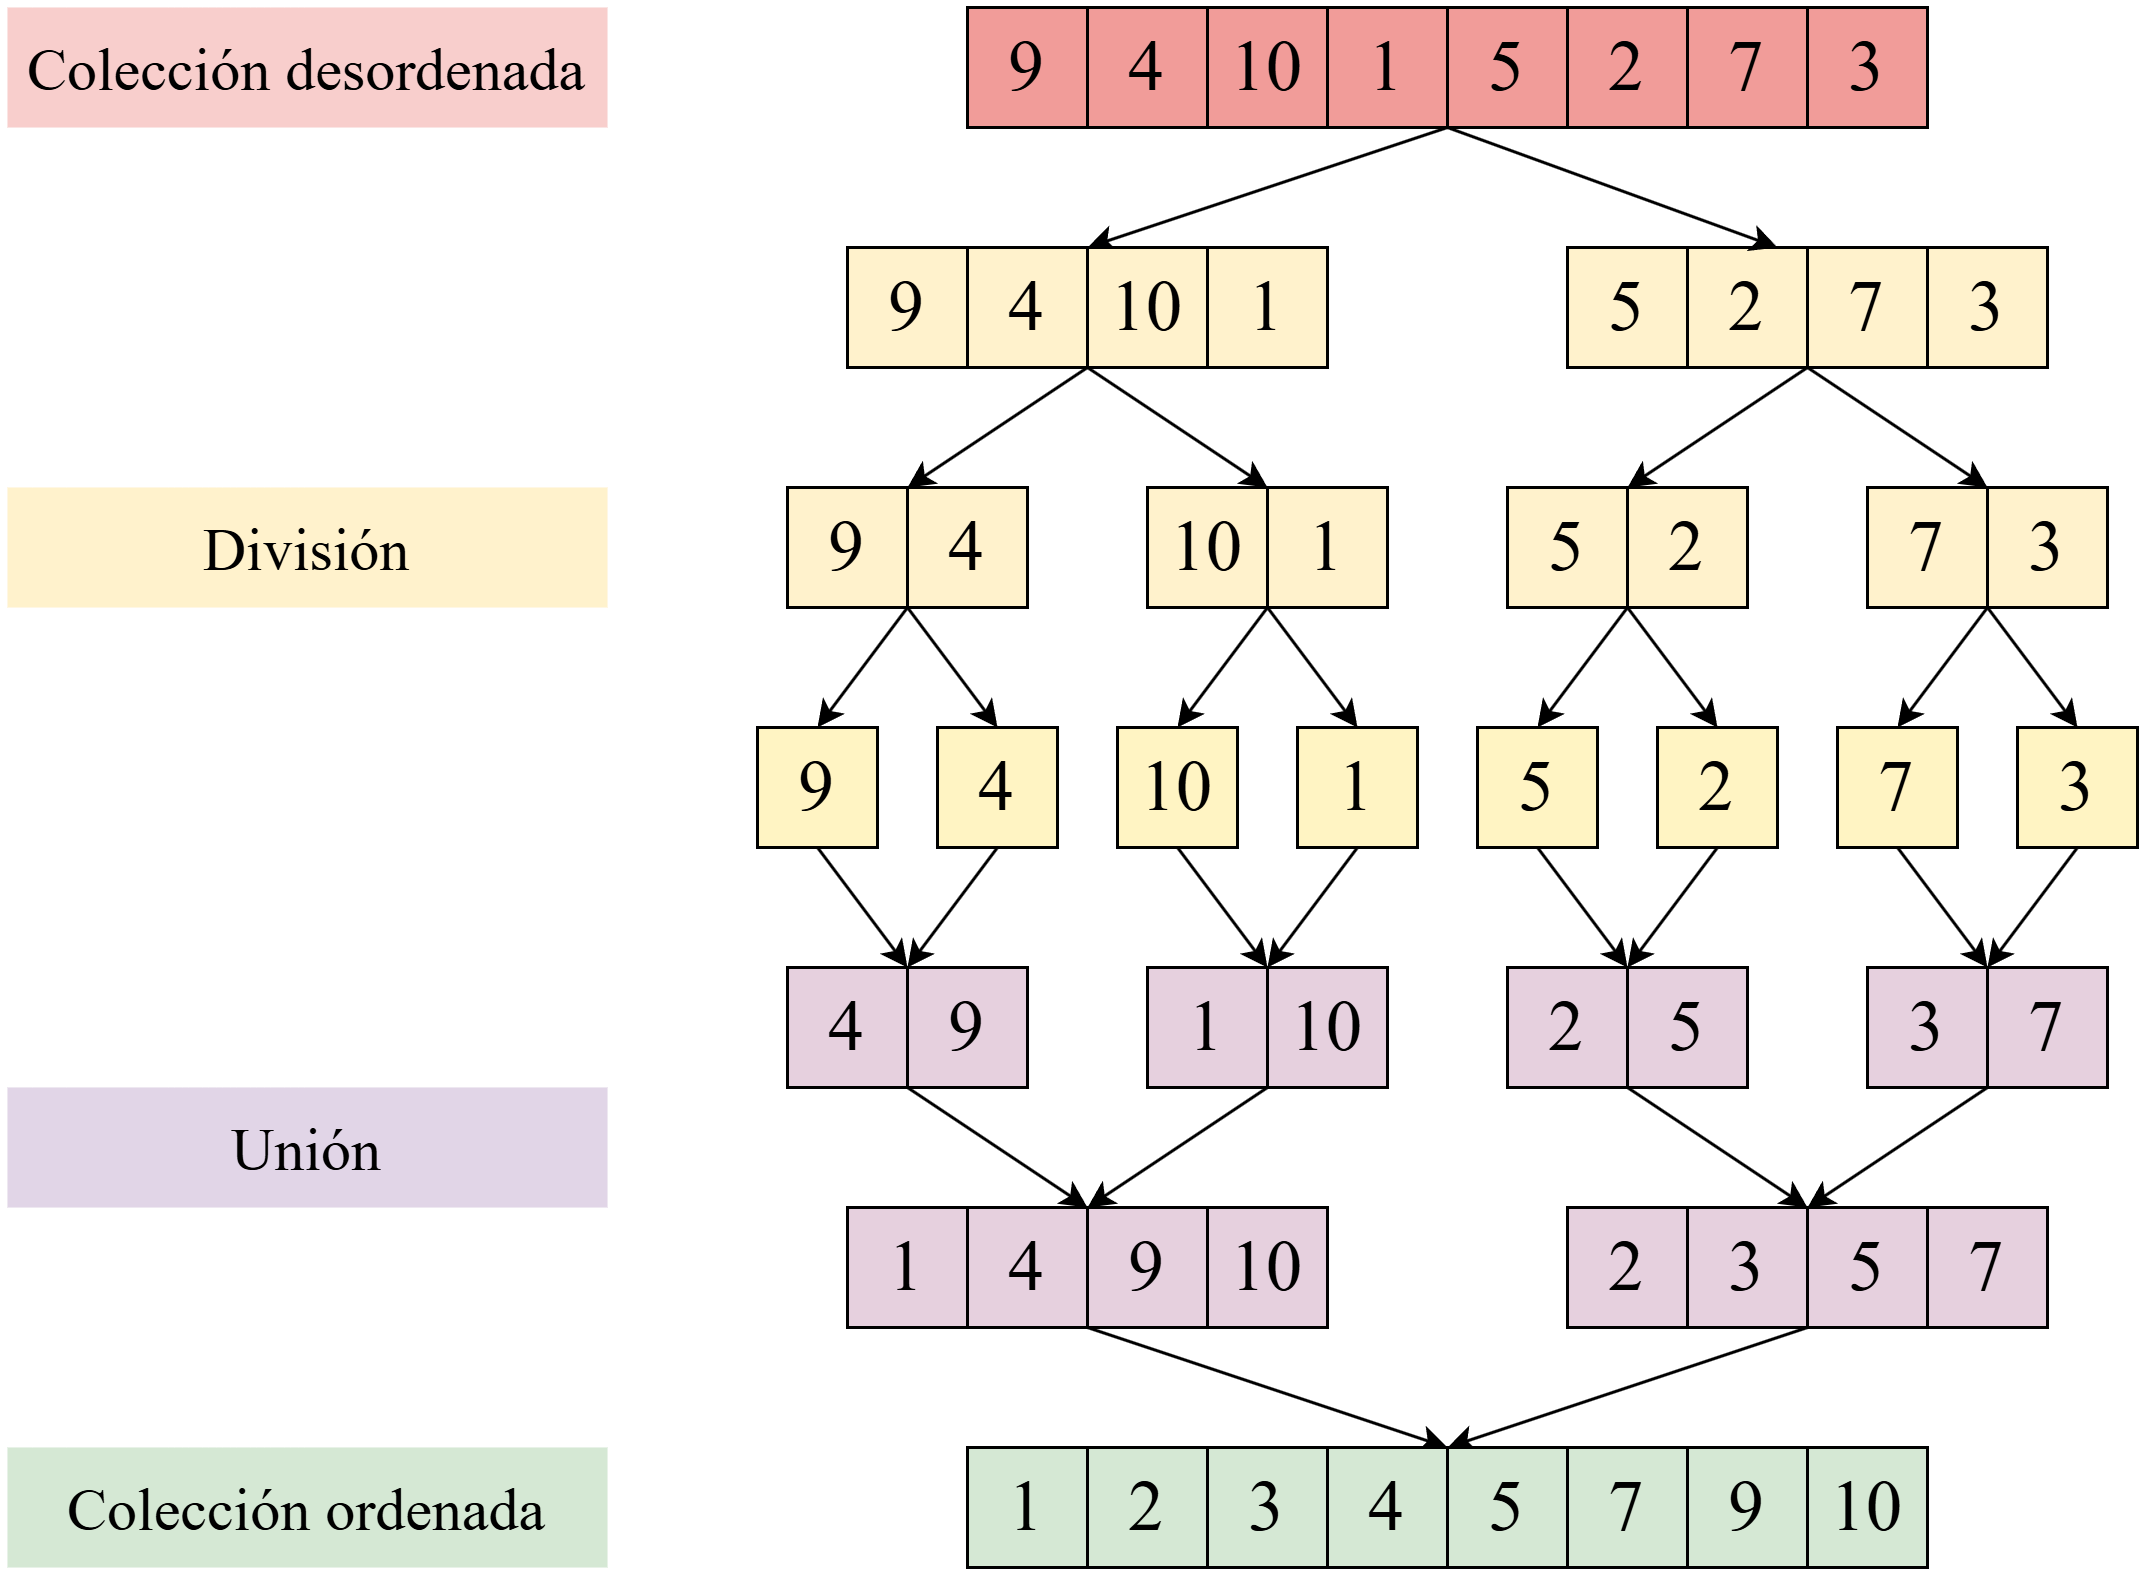
\includegraphics[width=0.50\linewidth]{Diagrames/arbolMS.png}
    \caption{Funcionamiento del \textit{Merge Sort}}
    \label{fig:arbolMS}
\end{figure}

\subsection{Ejecución serial y paralela}
Un \textbf{programa informático} es un conjunto de instrucciones que un sistema informático ejecuta. A su vez, un programa se divide en partes más pequeñas e independientes que llamamos tareas. Cuando las tareas se ejecutan una tras otra durante períodos de tiempo no superpuestos, hablamos de \textbf{ejecución serial}. A veces, la ejecución de una tarea depende del resultado de la tarea anterior. En dicho caso, la tarea bloquea a la siguiente. Esto es la \textbf{computación secuencial}. En contraposición, la \textbf{ejecución paralela} consiste en ejecutar varias tareas simultáneamente. Sin embargo, el paralelismo real solo es posible si el sistema consta de más de una unidad de procesamiento y si las tareas del algoritmo son independientes. \footnote{\cite{bobrov-2023}} Este estudio pretende aplicar el paralelismo a la ordenación por mezcla para aumentar la eficiencia del algoritmo.

%%76

\begin{figure}
    \centering
    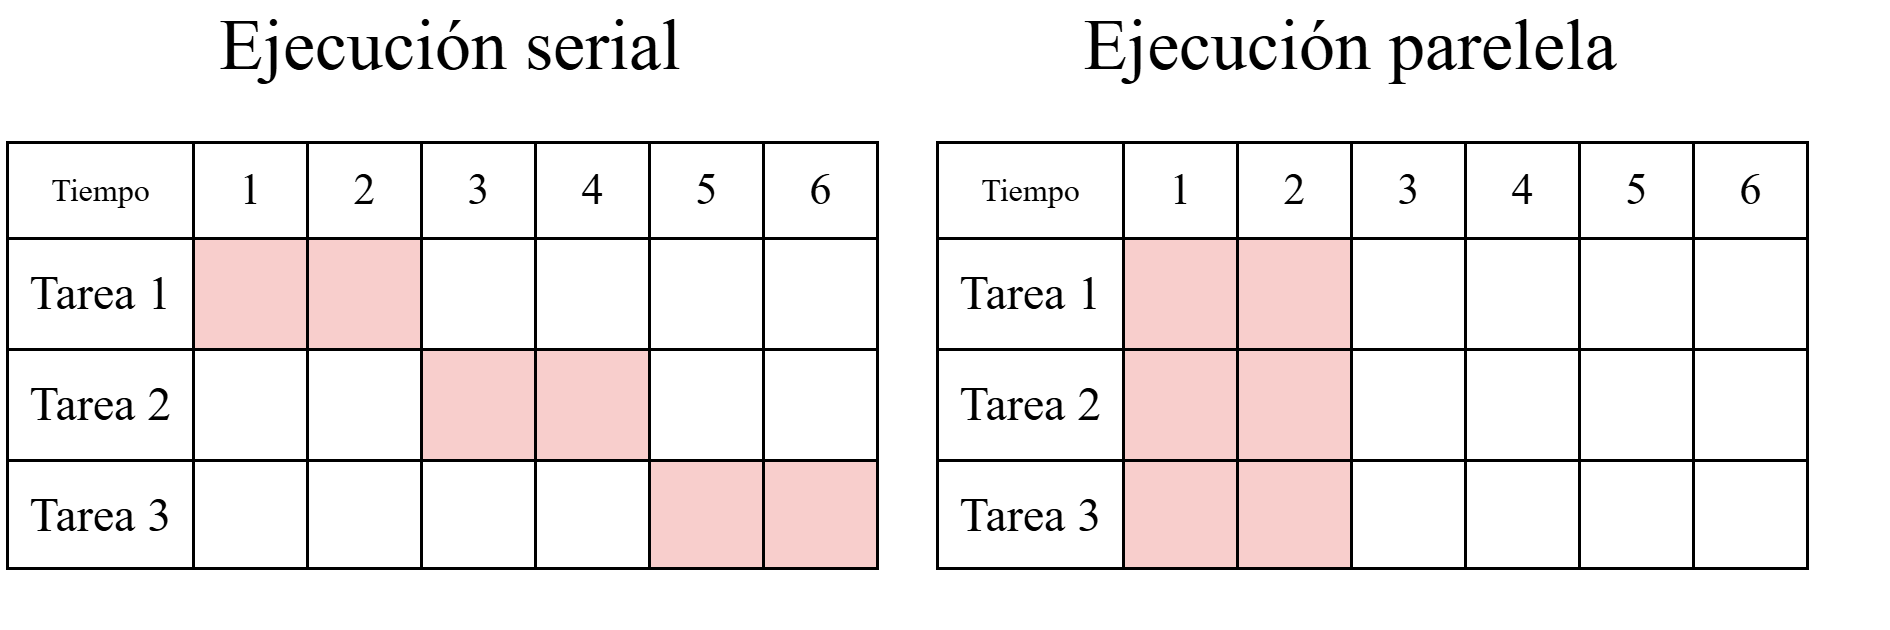
\includegraphics[width=0.65\linewidth]{Diagrames/serialVsParallel.png}
    \caption{Comparación de los diagramas de Gantt (//Nota: Probablemente cambiar por dos árboles mostrando la secuencia de instrucciones)}
    \label{fig:serialVsParallel}
\end{figure}

\subsection{Iteración y recursividad}
El paradigma de la \textbf{programación estructurada} considera que todo programa informático está formado por las estructuras de control de Secuencia, Selección y Repetición.\footnote{\cite{extended-learning-institute-no-date}} La recursión es una estructura de repetición.\footnote{\cite{wellesley-college-2000}} Si un programa incorpora una estructura recursiva, quiere decir que hay una función que se llama a sí misma. \footnote{\cite{bhargava-2016}} Toda función recursiva contiene caso recursivo, estructura condicional que llama a la propia función, y un caso base,  que retorna un valor constante o finaliza la función. 

%%

\textbf{[\\Nota: añadir gráfico para mostrar la recursión??]}

\subsection{Complejidad}
Esta investigación evalúa la aplicación de todos estos conceptos al algoritmo de ordenación por mezcla. La eficiencia de un algoritmo de ordenación usualmente se cuantifica en términos de complejidad temporal y espacial. La complejidad temporal es una medida de la variación del tiempo de ejecución de un algoritmo a medida que el tamaño de la entrada crece. El tiempo de ejecución se ve afectado por variables como el soporte físico y lógico (CPU\footnote{Central Processing Unit}, RAM\footnote{Random Access Memory}, lenguaje de programación, SO...)\footnote{\cite{Heineman2008-mw}} Es por ello, que se estudia el comportamiento asintótico de la complejidad, es decir, cuando el tamaño de la entrada $n$ tiende al infinito. Lo hace mediante las funciones del: peor caso posible \(O(n)\), el caso promedio \(\theta(n)\), y el mejor caso posible \(\Omega(n)\). \footnotemark[8] De ahí la notación \textit{Big-O}, que permite comparar algoritmos a través de distintas plataformas y predecir el tiempo de ejecución de un algoritmo.

La \textbf{complejidad temporal} se mide normalmente mediante la función del peor caso posible por varios motivos: es más sencillo de analizar al no ser necesario conocer la distribución de datos de entrada, garantiza el buen funcionamiento del programa en el que se incorpore en caso de situaciones desfavorables... (\\NOTA: Más ejemplos!!) Caracterizar un algoritmo mediante su complejidad \(O(n)\) es una abstracción, ya que se fundamenta en el modelo de Máquina de Acceso Aleatorio, que considera que las \textit{operaciones básicas}, como las aritméticas, lógicas o los accesos a la memoria, duran una sola unidad de tiempo. Asimismo, se considera que cada línea de código es una \textit{instrucción básica} que ejecuta un número constante de operaciones básicas. Los bucles (\lstinline{for}, \lstinline{for, while...}) y llamadas a funciones se evalúan sumando sus instrucciones básicas.

\begin{figure}[h]
	\captionsetup{justification=centering}
	\centering   
	
	\begin{tikzpicture}[scale=0.8]
		\begin{axis}[
			xlabel={Entrada $n$},
			ylabel={Tiempo de ejecución $y$}, 
			xmin=0, xmax=20, 
			ymin=0, ymax=100, 
			xtick={0,5,10,15,20,7},
			legend pos=north west, 
			grid=major,
			grid style={dashed, gray!30} 
			] 
			\addplot[ 
			domain=0:20, 
			samples=20, 
			color=blue,thick 
			]{4*x + 7}; 
			
			\addlegendentry{$f(n) = 4n + 7$} 
			\addplot[ 
			domain=0:20, 
			samples=20, 
			color=orange, thick 
			]{5*x}; 
			
			\addplot[ 
			color=black, dashed, thick 
			] coordinates{(7,0) (7,35)};
			
			\addlegendentry{$g(n) = 5n$} 
		\end{axis}
	\end{tikzpicture}
	
	\caption{Ejemplo de \textit{Big-O}}
	\label{fig:bigO}
\end{figure}

La notación \textit{Big-O} proporciona un límite superior para el cual una función nunca lo sobrepasará. Esta notación estudia el orden de crecimiento de una función. Formalmente, se define como: dadas dos funciones \(f(n)\), \(g(n)\), entonces \(f(n) = O(g(n))\) siempre que existan las constantes \(c\) y \(n_0\) tal que \(f(n) \leq c\cdot g(n)\), para todo \(n \geq n_0\). Esto significa que para una función \(f(n)\) solo existirá un Big-O \(O(g(n))\) si todos los valores de su entrada \(n\) son inferiores al producto entre una constante \(c\) y una función \(g(n)\), que es el límite superior. De forma que, \(f(n)\) nunca crecerá más que \(g(n)\).

Por ejemplo, se da un algoritmo que toma un tiempo de ejecución \(f(n) = 4n+7\) y queremos saber si se comporta de forma lineal. Esto es \(g(n)=n\) Entonces para que \(f(n) = O(g(n))\) hay que encontrar un valor de \(c\) para el que se cumpla que \(4n+7 \leq c\cdot n\). Con \(c=5\) la inecuación se cumple, por tanto: \(f(n) = O(g(n)) = O(n)\); y esto solo se cumple para \(n \geq n_0\), en este caso \(n\geq 7\) porque: \(4n+7 \leq 5n \space \rightarrow 7 \leq 5n - 4n   \rightarrow 7 \leq n\). De forma que el \textit{Big-O} de \(4n+7\) es \(O(n)\) para cualquier entrada mayor que \(7\).


\newpage
\section{Implementaciones}

\subsection{Merge Sort Recursivo Serial (MSRS)}
El algoritmo de ordenación por mezcla clásico se basa en el paradigma <<divide y vencerás>>. Es decir, primero se divide un problema en otros subproblemas, se solucionan los subproblemas, y, se combinan para llegar a la solución
final.\footnote{\cite{Sedgewick2003-cd}}

\begin{figure}[h]
    \begin{lstlisting}[language=java, frame=single, numbers=left]
public static void sort(int[] arr, int[] aux, int left, int right) {
	if (left >= right) return;
	
	int mid = left + (right - left) / 2;
	
	sort(arr, aux, left, mid);
	sort(arr, aux,mid+1, right);
	
	merge(arr, aux, left, mid, right);
}
    \end{lstlisting}
    \caption{Función \lstinline{sort()} del Merge Sort Recursivo Serial}
    \label{fig:MSRS_sort()}
\end{figure}

El algoritmo a estudiar consta de una función \lstinline{sort()} que toma una colección \lstinline{arr}, un índice inicial \lstinline{left} y un índice final \lstinline{right}. (Véase la Figura \ref{fig:MSRS_sort()}) Después calcula el pivote \lstinline{mid} desde donde dividir la colección original \lstinline{arr[]} y se ejecuta una llamada recursiva a \lstinline{sort()} para cada mitad \lstinline{arr[left]... arr[mid]} y \lstinline{arr[mid+1]... arr[right]}.

\begin{figure}[h]
    \begin{lstlisting}[language=java, frame=single, numbers=left]
private static void merge(int[] arr, int[] aux, int left, int mid, int right) {
	for (int i = left; i <= right; i++) aux[i] = arr[i];
	
	int i = left, j = mid + 1, k = left;
	
	while (i <= mid && j <= right) arr[k++] = (aux[i] <= aux[j])? aux[i++] : aux[j++];
	
	while (i <= mid) arr[k++] = aux[i++];
}
    \end{lstlisting}
    \caption{Función \lstinline{merge()} del Merge Sort Recursivo Serial}
    \label{fig:MSRS_merge()}
\end{figure}

Finalmente, se unen las mitades mediante la función \lstinline{merge()} de la Figura \ref{fig:MSRS_merge()} que toma los mismos argumentos que \lstinline{sort()}, además del parámetro \lstinline{mid}. Para controlar el recorrido de las tres colecciones se emplean tres índices: \lstinline{i} para la midad izquierda \lstinline{arr[left]... arr[mid]}, \lstinline{j} para la mitad derecha \lstinline{arr[mid+1]... arr[right]} y \lstinline{k} para el arreglo original \lstinline{arr[left]... arr[right]}. Un primer bucle copia en un arreglo auxiliar \lstinline{aux[]} todos los elementos de \lstinline{arr[]}. Después, un segundo bucle recorre simultáneamente las dos mitades y la colección auxiliar; mientras coloca en \lstinline{arr[k]} el elemento más pequeño entre \lstinline{aux[i]} y \lstinline{aux[j]}. Existen dos posibilidades: primera, que el bucle se detenga porque \lstinline{i>mid}, que implica que todos los elementos de la primera mitad \lstinline{aux[left]... arr[mid]} han sido copiados en \lstinline{arr[]}; segunda, que el bucle se detenga porque \lstinline{j > right}, que implica que todos los elementos de la segunda mitad \lstinline{aux[mid+1]... arr[right]} han sido copiado en \lstinline{arr[]}. Sin embargo, si \lstinline{i} no alcanza \lstinline{mid} quedan elementos sin copiar en \lstinline{arr[]}: entonces un tercer bucle copia los elementos restantes de \lstinline{aux[i]... aux[mid]} en \lstinline{arr[]}.

Todas las implementaciones (MSRS, MSIS, MSRP, MSIP) emplean el mismo método \lstinline{merge()} para unir las sucesivas mitades.

\subsubsection{Complejidad}
La complejidad temporal del algoritmo será la suma de las complejidades de cada línea. Según el modelo MAN\footnote{Máquina de Acceso Aleatorio}, la comprobación del caso base (línea 2, Figura \ref{fig:MSRS_sort()}) y el cálculo del pivote \lstinline{mid} toman tiempo constante \(O(1)\) al ser operaciones básicas. La inicialización de \lstinline{L} y \lstinline{R} toma tiempo \(O(n)\) porque en Java la creación de un arreglo implica la asignación de espacio en la memoria proporcional al tamaño de este, en este caso \lstinline{lenght = }\(n\). La copia de las sub-colecciones (bucles de las líneas 8-9) toman \(O(n)\) al su tiempo de ejecución depender de \(n\). Por último, \lstinline{merge} (Figura \ref{fig:MSRS_merge()}) toma \(O(n)\) porque en el peor caso se realizaran \lstinline{left} \(+\) \lstinline{right} \(=\) \lstinline{lenght} comparaciones \lstinline{L[i]<=R[j]}, que es lo mismo que \(n\). Por tanto, el tiempo de ejecución respecto la entrada por ahora es \(f(n) = 2O(1) + 2O(n) + 2O(n)+ O(n)\), que es igual a \(O(n)\) ya que según la notación \textit{Big-O} se ignoran los términos de menor orden y los factores constantes, puesto que estos no afectan significativamente al crecimiento cuando \(n\) tiende a un número grande.

\begin{figure}[hbtp]
    \centering
    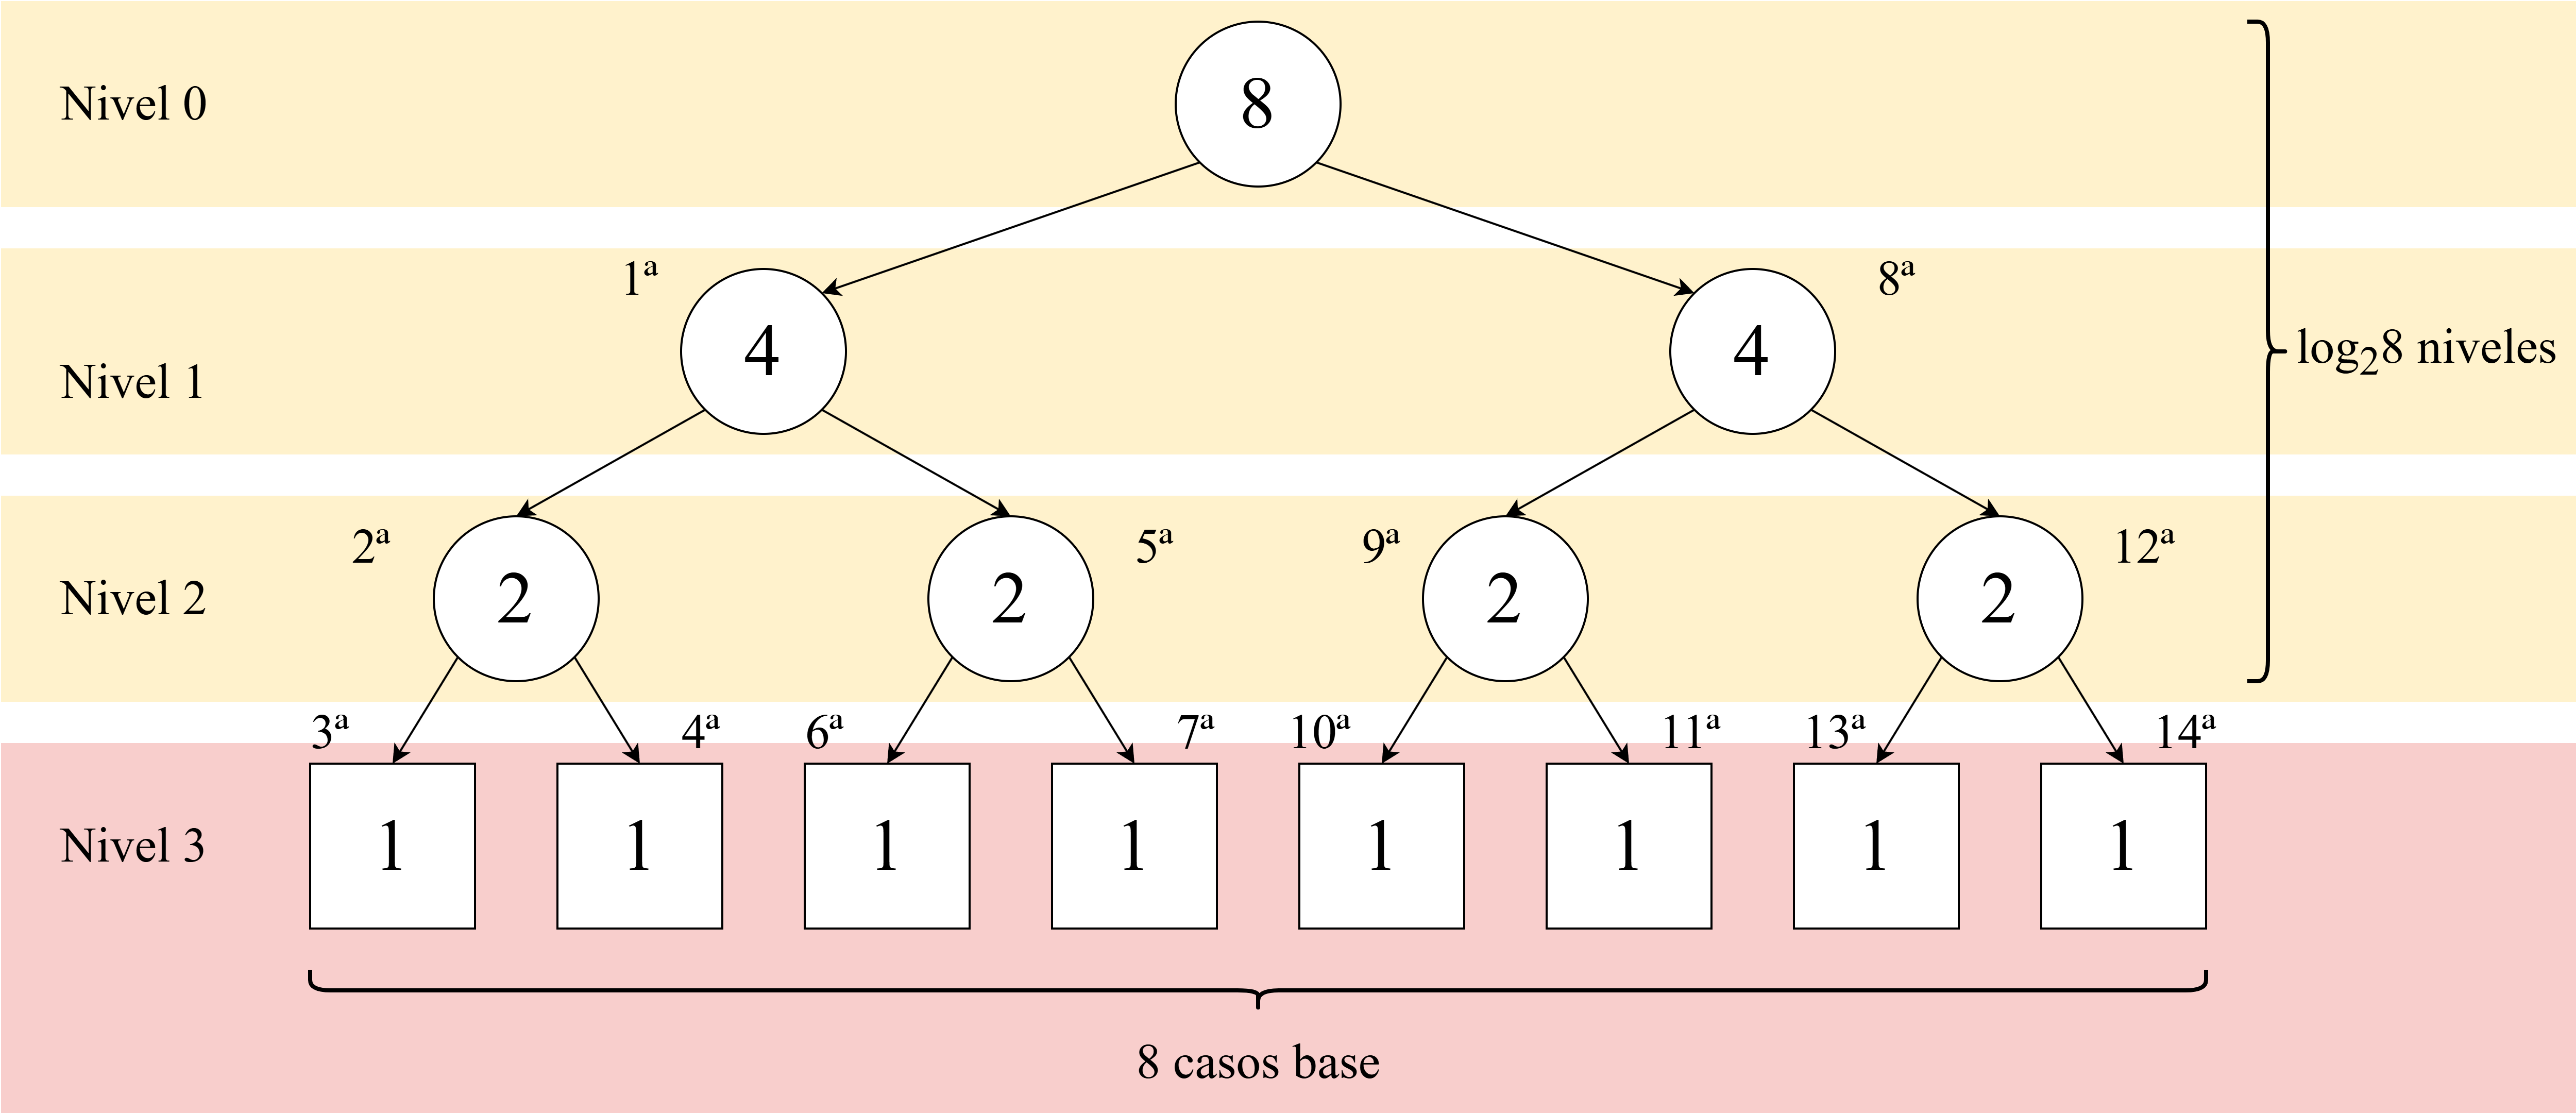
\includegraphics[width=0.8\linewidth]{Diagrames/arbolBinarioMSRSn8.png}
    \caption{Árbol binario para \(n=8\)}
    \label{fig:arbol-MSRS-N=8}
\end{figure}

Lo anterior corresponde a una llamada a \lstinline{sort()}, pero esta función es recursiva, por tanto, hay que determinar cuantas veces se llama a \lstinline{sort()} en función del tamaño de la entrada \(n\). Estos se facilita si rastreamos las llamadas a \lstinline{sort()}, por ejemplo mediante un árbol binario como el de la Figura \ref{fig:arbol-MSRS-N=8} donde cada nodo representa la longitud de la entrada \lstinline{lenght}. Se observa que para 8 llamadas hay tres niveles en el árbol, la relación entre 8 y 3 es que \(log_{2}{3} = 3\) ya que \(8=2^3\). Por extensión, para un \(n\) tamaño de entrada hay \(\log_{2}{n}\) niveles. Esto se cumple siempre que \(n\) sea múltiplo de 2, lo que da lugar a un árbol balanceado como el de Figura \ref{fig:simetriaMSRS}, en caso contrario está desbalanceado y hay llamadas extras. El trabajo realizado en cada nivel \(i\) es \(2^i\cdot n \cdot \frac{n}{2^i} = n\) como se observa en la Figura \ref{fig:entradaMSRS} donde \(n\) es el tamaño de entrada original. Finalmente, el trabajo \(f(n)\) de una llamada a \lstinline{sort()} es la suma del trabajo en cada nivel, menos el del último nivel porque los casos bases requieren \(O(1)\) al realizarse un \lstinline{return}. Esto es:
\[f(n) = \sum_{i=0}^{\log_{2}{n} -1} {n} = n\sum_{i=0}^{\log_{2}{n} -1} {1} = n\cdot\log_{2}{n}\]
A continuación se aplica la definición de la notación \textit{Big-0}, donde \(f(n)=n\log_{2}{n}\) y \(g(n)=n\log{n}\). Existe un \(f(n)=O(n\log{n})\) siempre que: 
\[n\log_{2}{n} \leq c\cdot n\log{n}\]
Aislamos la constante \(c\):
\[n\log_{2}{n} \leq c\cdot n\log{n} \longrightarrow c \geq \frac{\log_{2}{n}} {\log_{10}{n}} \longrightarrow c \geq \frac{ \frac{\log_{10}{n}} {\log_{10}{2}} } {\log_{10}{n}} \longrightarrow c \geq \frac{1}{\log{2}} \]
Esto significa que la complejidad del MSRS se aleja de \(O(n\log_n)\) en un factor aproximado de \(3,32\%\) siempre que la entrada sea mayor que 1 y sea múltiplo de 2. Aun así, la literatura considera que el \textit{Merge Sort} tiene complejidad \(O(n\log{n})\) por razones prácticas. \footnote{\cite{Sedgewick2003-cd}}

\begin{figure}[h]
\centering 
\captionsetup{justification=centering, margin=10pt}
\begin{minipage}{0.5\textwidth} 
    \centering 
    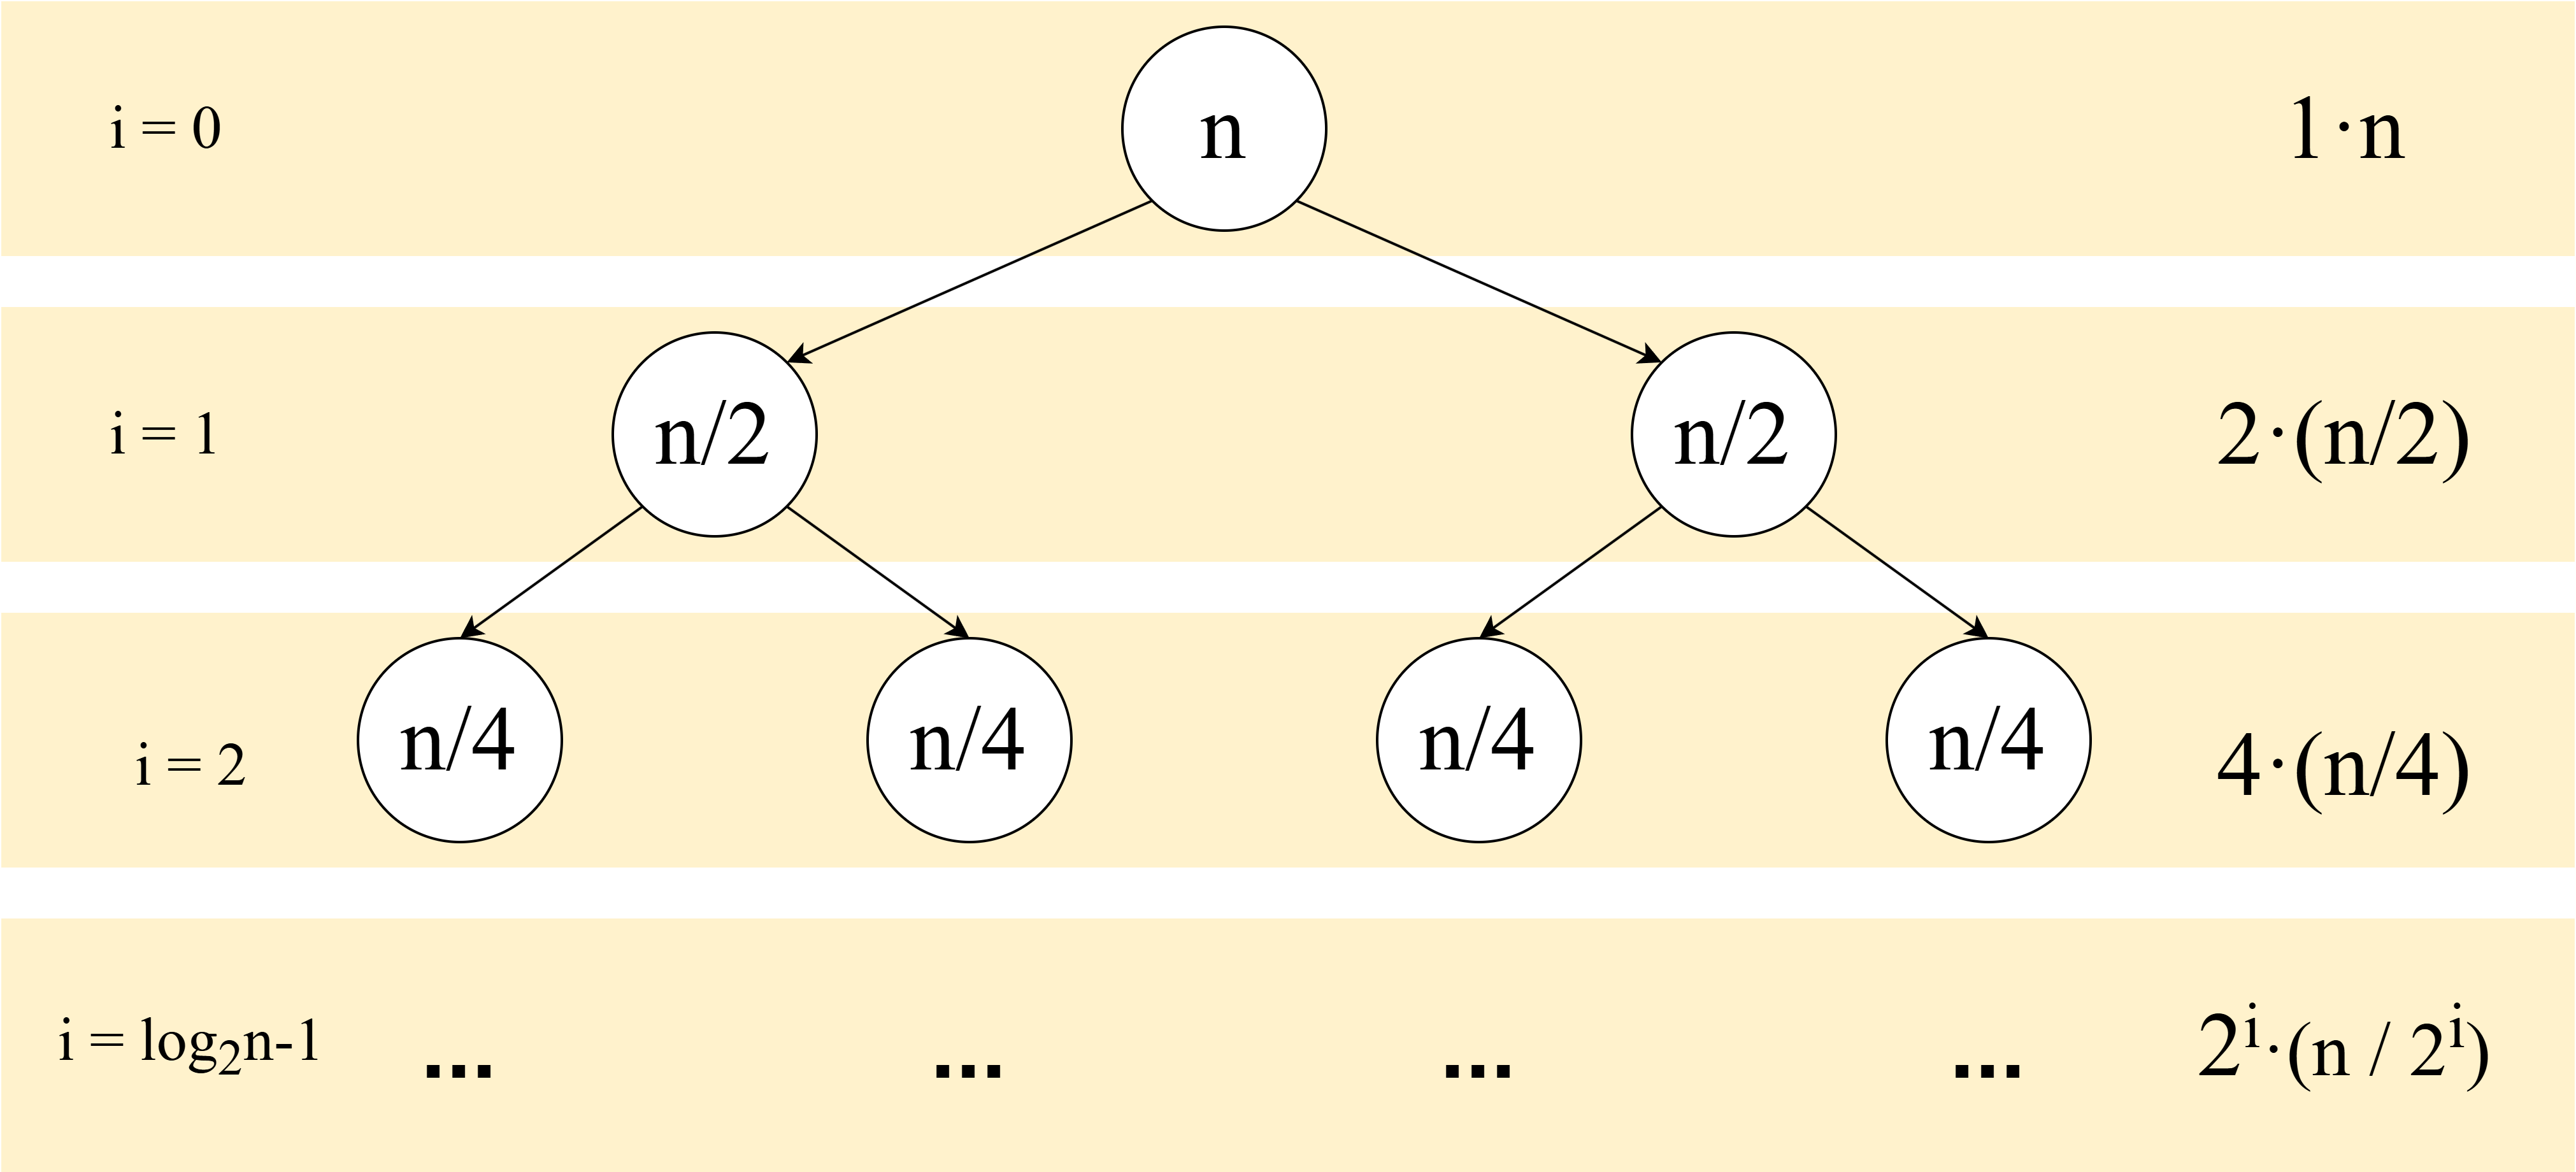
\includegraphics[width=0.95\linewidth]{Diagrames/arbolBinarioLenght.png} 
    \caption{Tamaño de la entrada a lo largo de las llamadas a \lstinline{sort()}} 
    \label{fig:entradaMSRS}
\end{minipage}\hfill 
\begin{minipage}{0.5\textwidth} 
    \centering 
    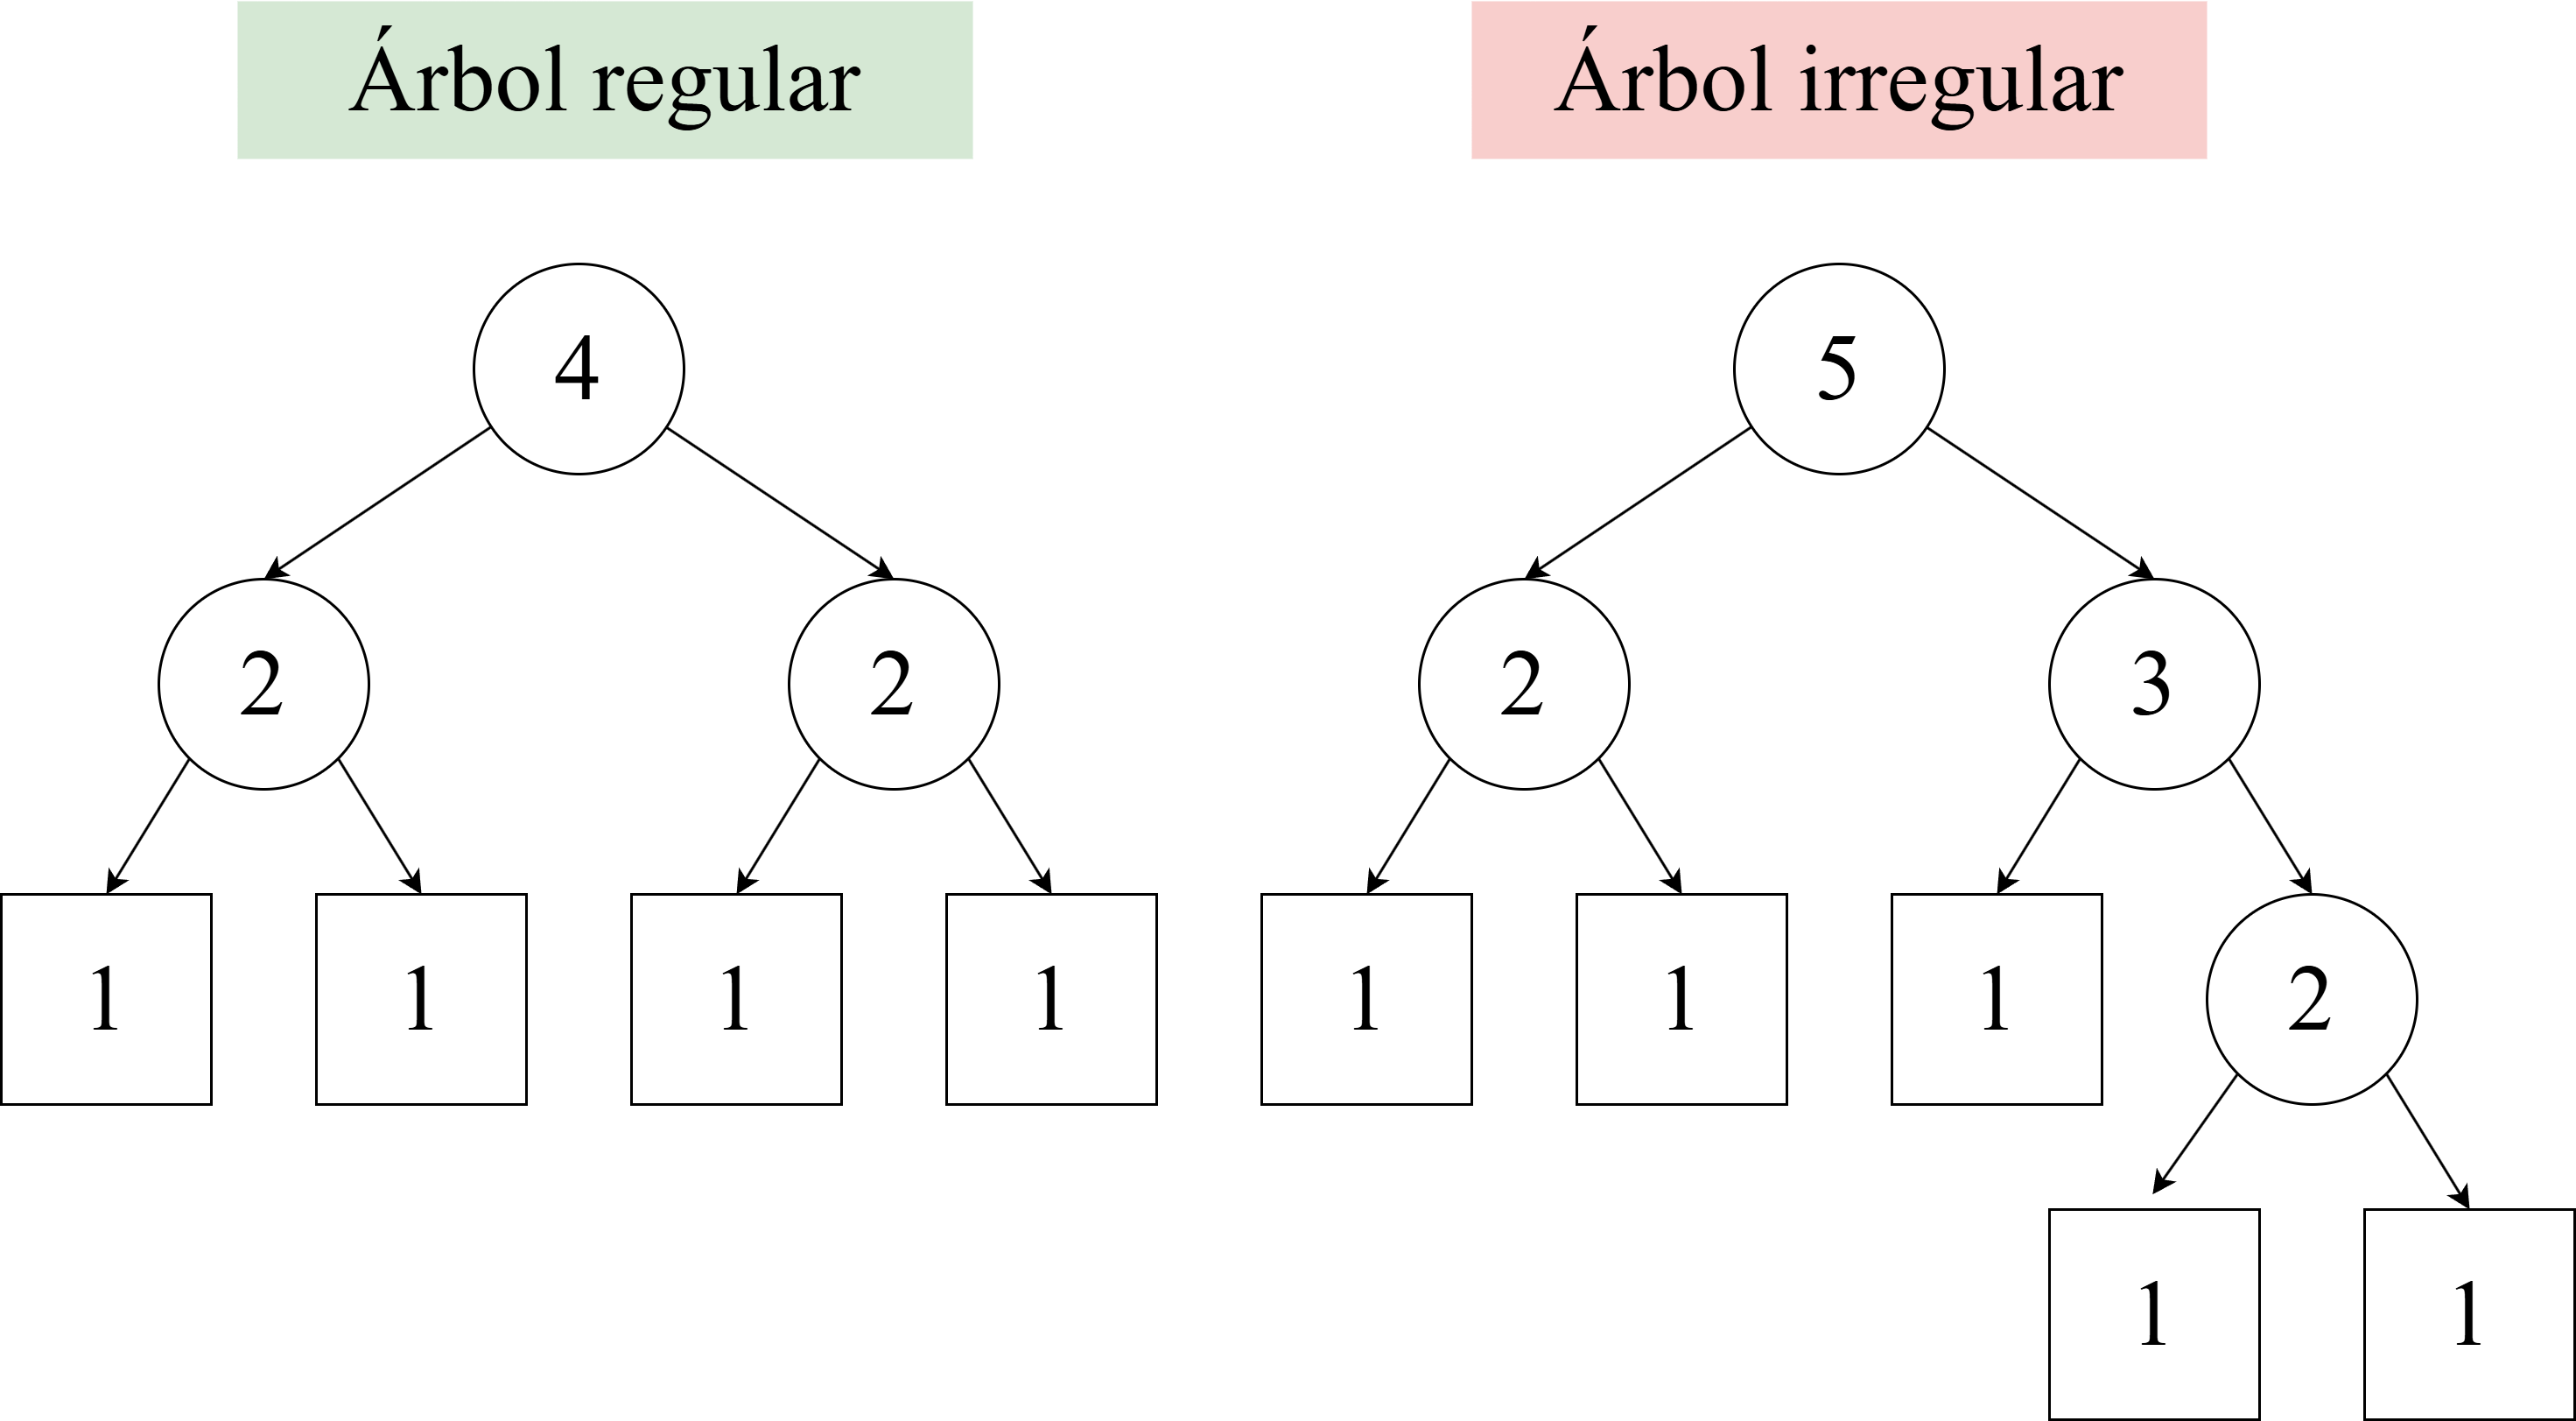
\includegraphics[width=0.95\linewidth]{Diagrames/arbolBinario_MSRS.png} 
    \caption{Árbol balanceado versus árbol desbalanceado del MSRS} 
    \label{fig:simetriaMSRS}
\end{minipage} \end{figure}

\subsection{Merge Sort Iterativo Serial (MSIS)}

El MSIS es la versión análoga al clásico MSRS, en esta implementación (Figura \ref{fig:MSIS_sort()}) se divide la colección en partes más pequeñas, después las partes adyacentes se unen, y se aumenta el tamaño  de las partes. Estos tres pasos se repiten hasta que la parte tenga el tamaño de la colección original. El primer bucle determina el tamaño \lstinline{lenght} de las partes: \lstinline{size} \(=2, 4, 8..\). El segundo bucle determina el índice \lstinline{left} desde el cual comienza la parte \lstinline{arr[left]...arr[left+size-1]} que será unida a su adyacente \lstinline{arr[mid]...arr[right]} mediante \lstinline{merge()}. Este índice toma valores en intervalos de \lstinline{2*size}. En la Figura \ref{fig:ejecuciónMSIS} se presenta el proceso de ordenación de una colección: las casillas coloreadas representan las sucesivas iteraciones de \lstinline{left} del segundo bucle; las casillas azules corresponden a la respectiva parte izquierda de una iteración; y las verdes la parte derecha.

\begin{figure}[hbtp]
    \begin{lstlisting}[language=java, frame=single, numbers=left]
public static void sort(int[] arr, int[] aux) {
	int n = arr.length;
	
	for (int size = 1; size < n; size *= 2) {
		for (int left = 0; left < n - size; left += 2 * size) {
			int mid = left + size - 1;
			int right = Math.min(left + 2 * size - 1, n - 1);
			merge(arr, aux, left, mid, right);
		}
	}
}
    \end{lstlisting}
    \caption{Función \lstinline{sort()} del Merge Sort Iterativo Serial}
    \label{fig:MSIS_sort()}
\end{figure}

\begin{figure}
    \centering
    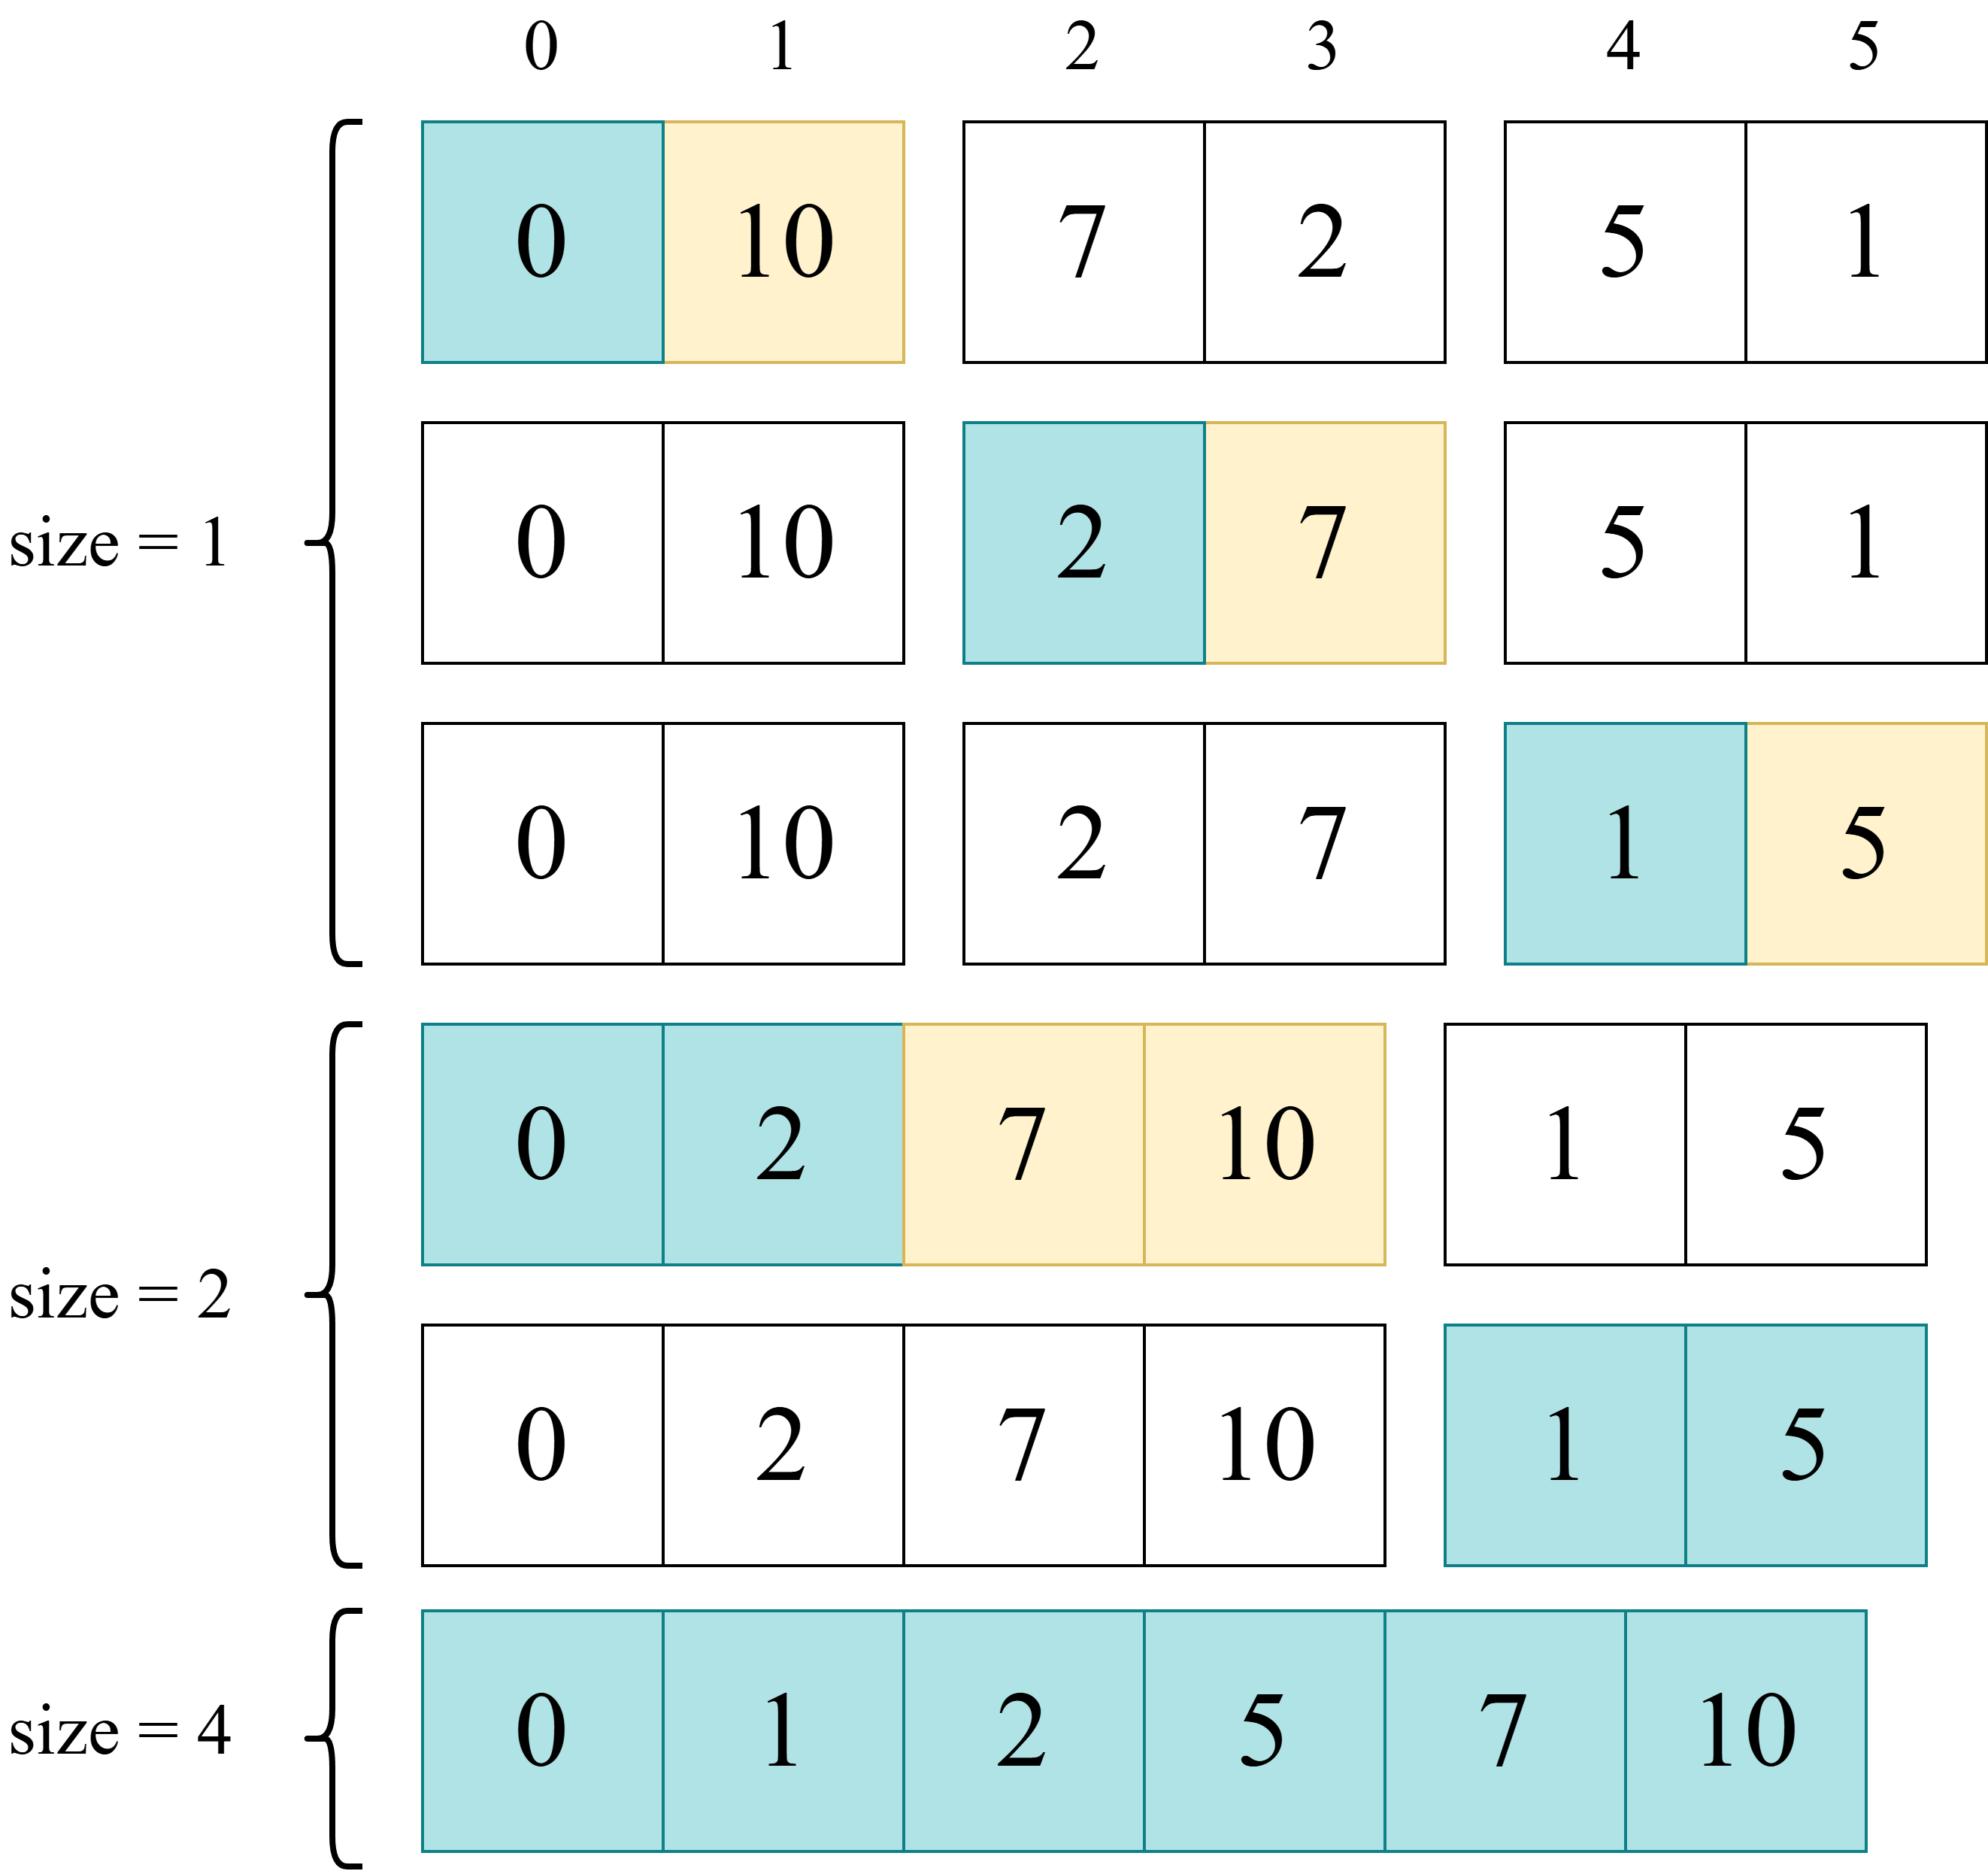
\includegraphics[width=0.5\linewidth]{Diagrames/ejecucionMSIS.png}
    \caption{Ejecución del Merge Sort Iterativo Serial}
    \label{fig:ejecuciónMSIS}
\end{figure}

\subsubsection{Complejidad temporal}
El MSIS recorre el árbol (véase la Figura \ref{fig:arbolMSIS}) desde la base de la recursión hasta la parte superior, ya que se realizan uniones entre partes de longitud 1-1, 2-2- 4-4... Como en el MSRS, el árbol será balanceado solo si el tamaño de entrada es múltiplo de 2. Siguiendo el mismo método y tomando las mismas suposiciones que en el cálculo de la complejidad temporal del MSRS, la complejidad del MSRS es \(O(n \log{n})\) porque hay \(\log_2{n}-1\) llamadas a \lstinline{sort()} en las cuales se realiza un trabajo de \(O(n)\) en el peor caso.

\begin{figure}
    \centering
    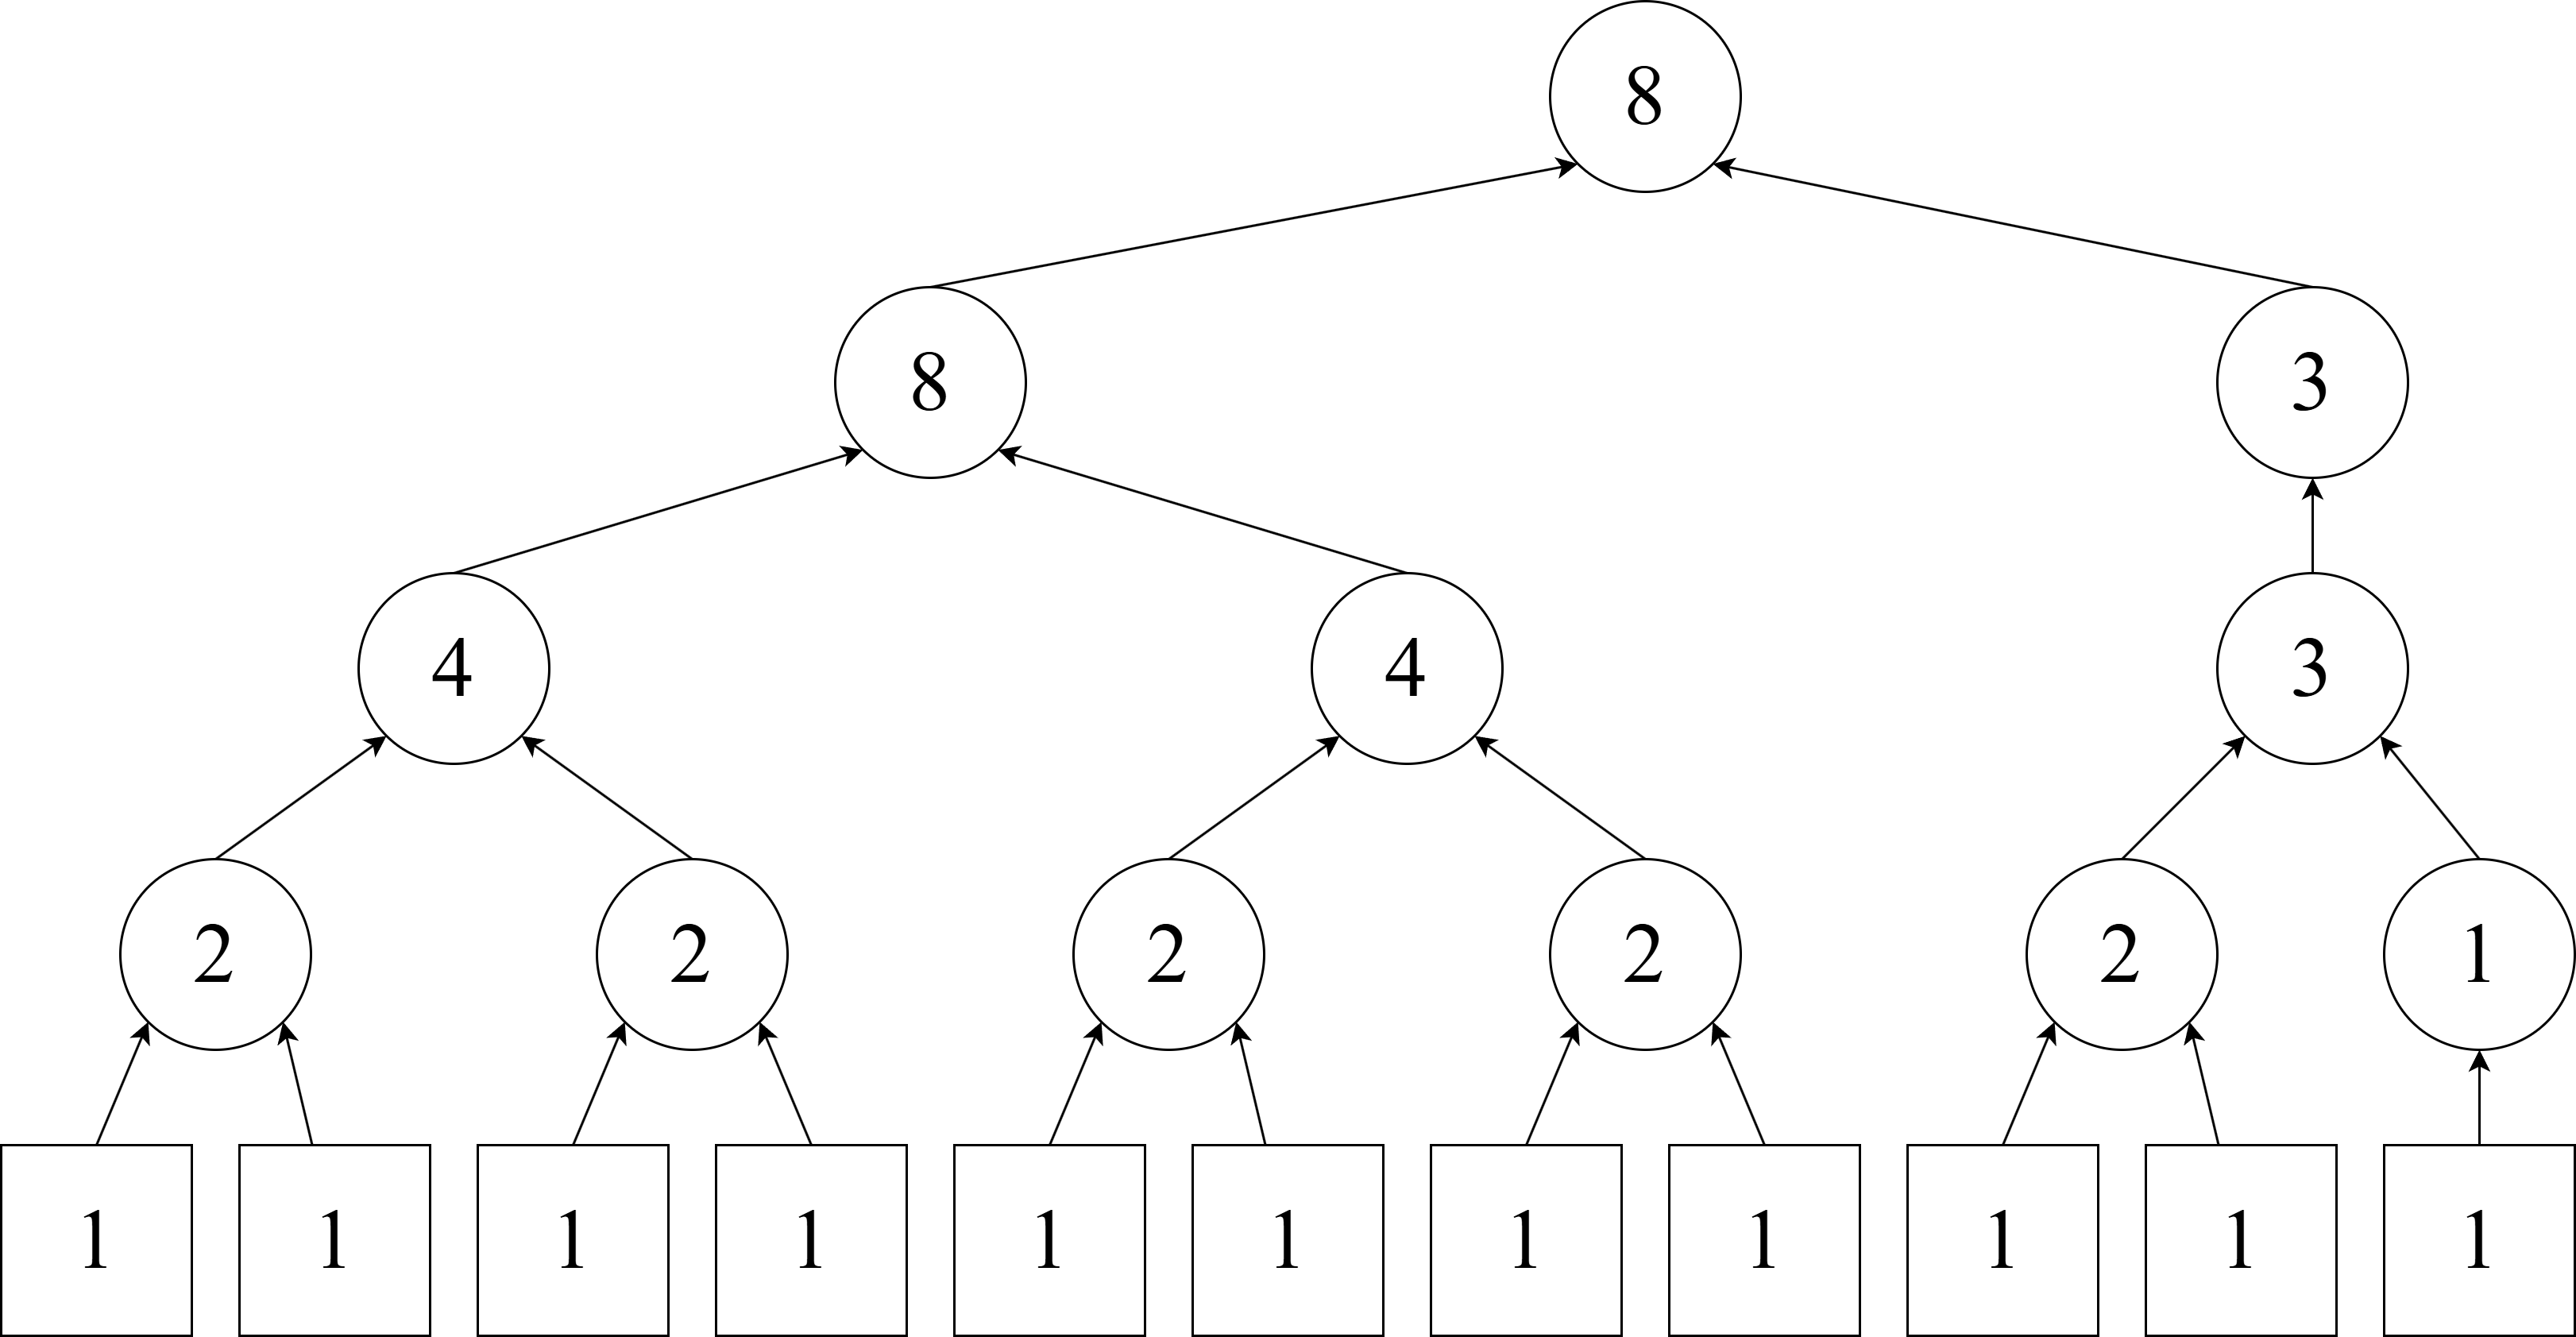
\includegraphics[width=0.7\linewidth]{Diagrames/arbolMSISirregular.png}
    \caption{Árbol binario del Merge Sort Iterativo Serial}
    \label{fig:arbolMSIS}
\end{figure}


\newpage
\subsection{Merge Sort Recursivo Paralelo (MSRP)}
Un proceso es la ejecución de las instrucciones de un programa; después de que estas instrucciones se hayan movido desde la memoria secundaria (SSD\footnote{\textit{Solid-state drive}} por ejemplo) hasta la primaria (RAM\footnote{\textit{Random access memory}}). El sistema operativo crear los procesos y guarda en la memoria su información asociada: el un identificador de proceso único (\textit{PID}); un espacio de direcciones de memoria, ya que un proceso lee y modifica datos guardados en la memoria; el estado del proceso; y, una lista de los archivos que el programa usa. En cambio, un hilo de ejecución es una secuencia de instrucciones que el planificador del sistema operativo puede manejar independientemente. \footnote{\cite{bobrov-2023}} Hasta el momento se han mostrado programas que al ejecutarse toman la forma de un proceso con un solo hilo de ejecución (MSIS y MSRS). La idea es mejorar el rendimiento del \textit{Merge Sort} haciendo uso de más de un hilo de ejecución. 

La herramienta más apropiada que proporciona Java para este problema es la clase \lstinline{ForkJoinPool}.\footnotemark \footnotetext{\cite{OracleForkJoin}} Una piscina de hilos (\textit{thread pool}), es un espacio en el que se mantienen un conjunto fijo de hilos de ejecución reutilizables que esperan a que se les pase un conjunto de instrucciones a ejecutar. Una piscina evita la necesidad de crear y destruir hilos constantemente, hecho que conlleva un costo computacional elevado.\footnote{\cite{engle_2022}}

\begin{figure}[h]
	\centering
	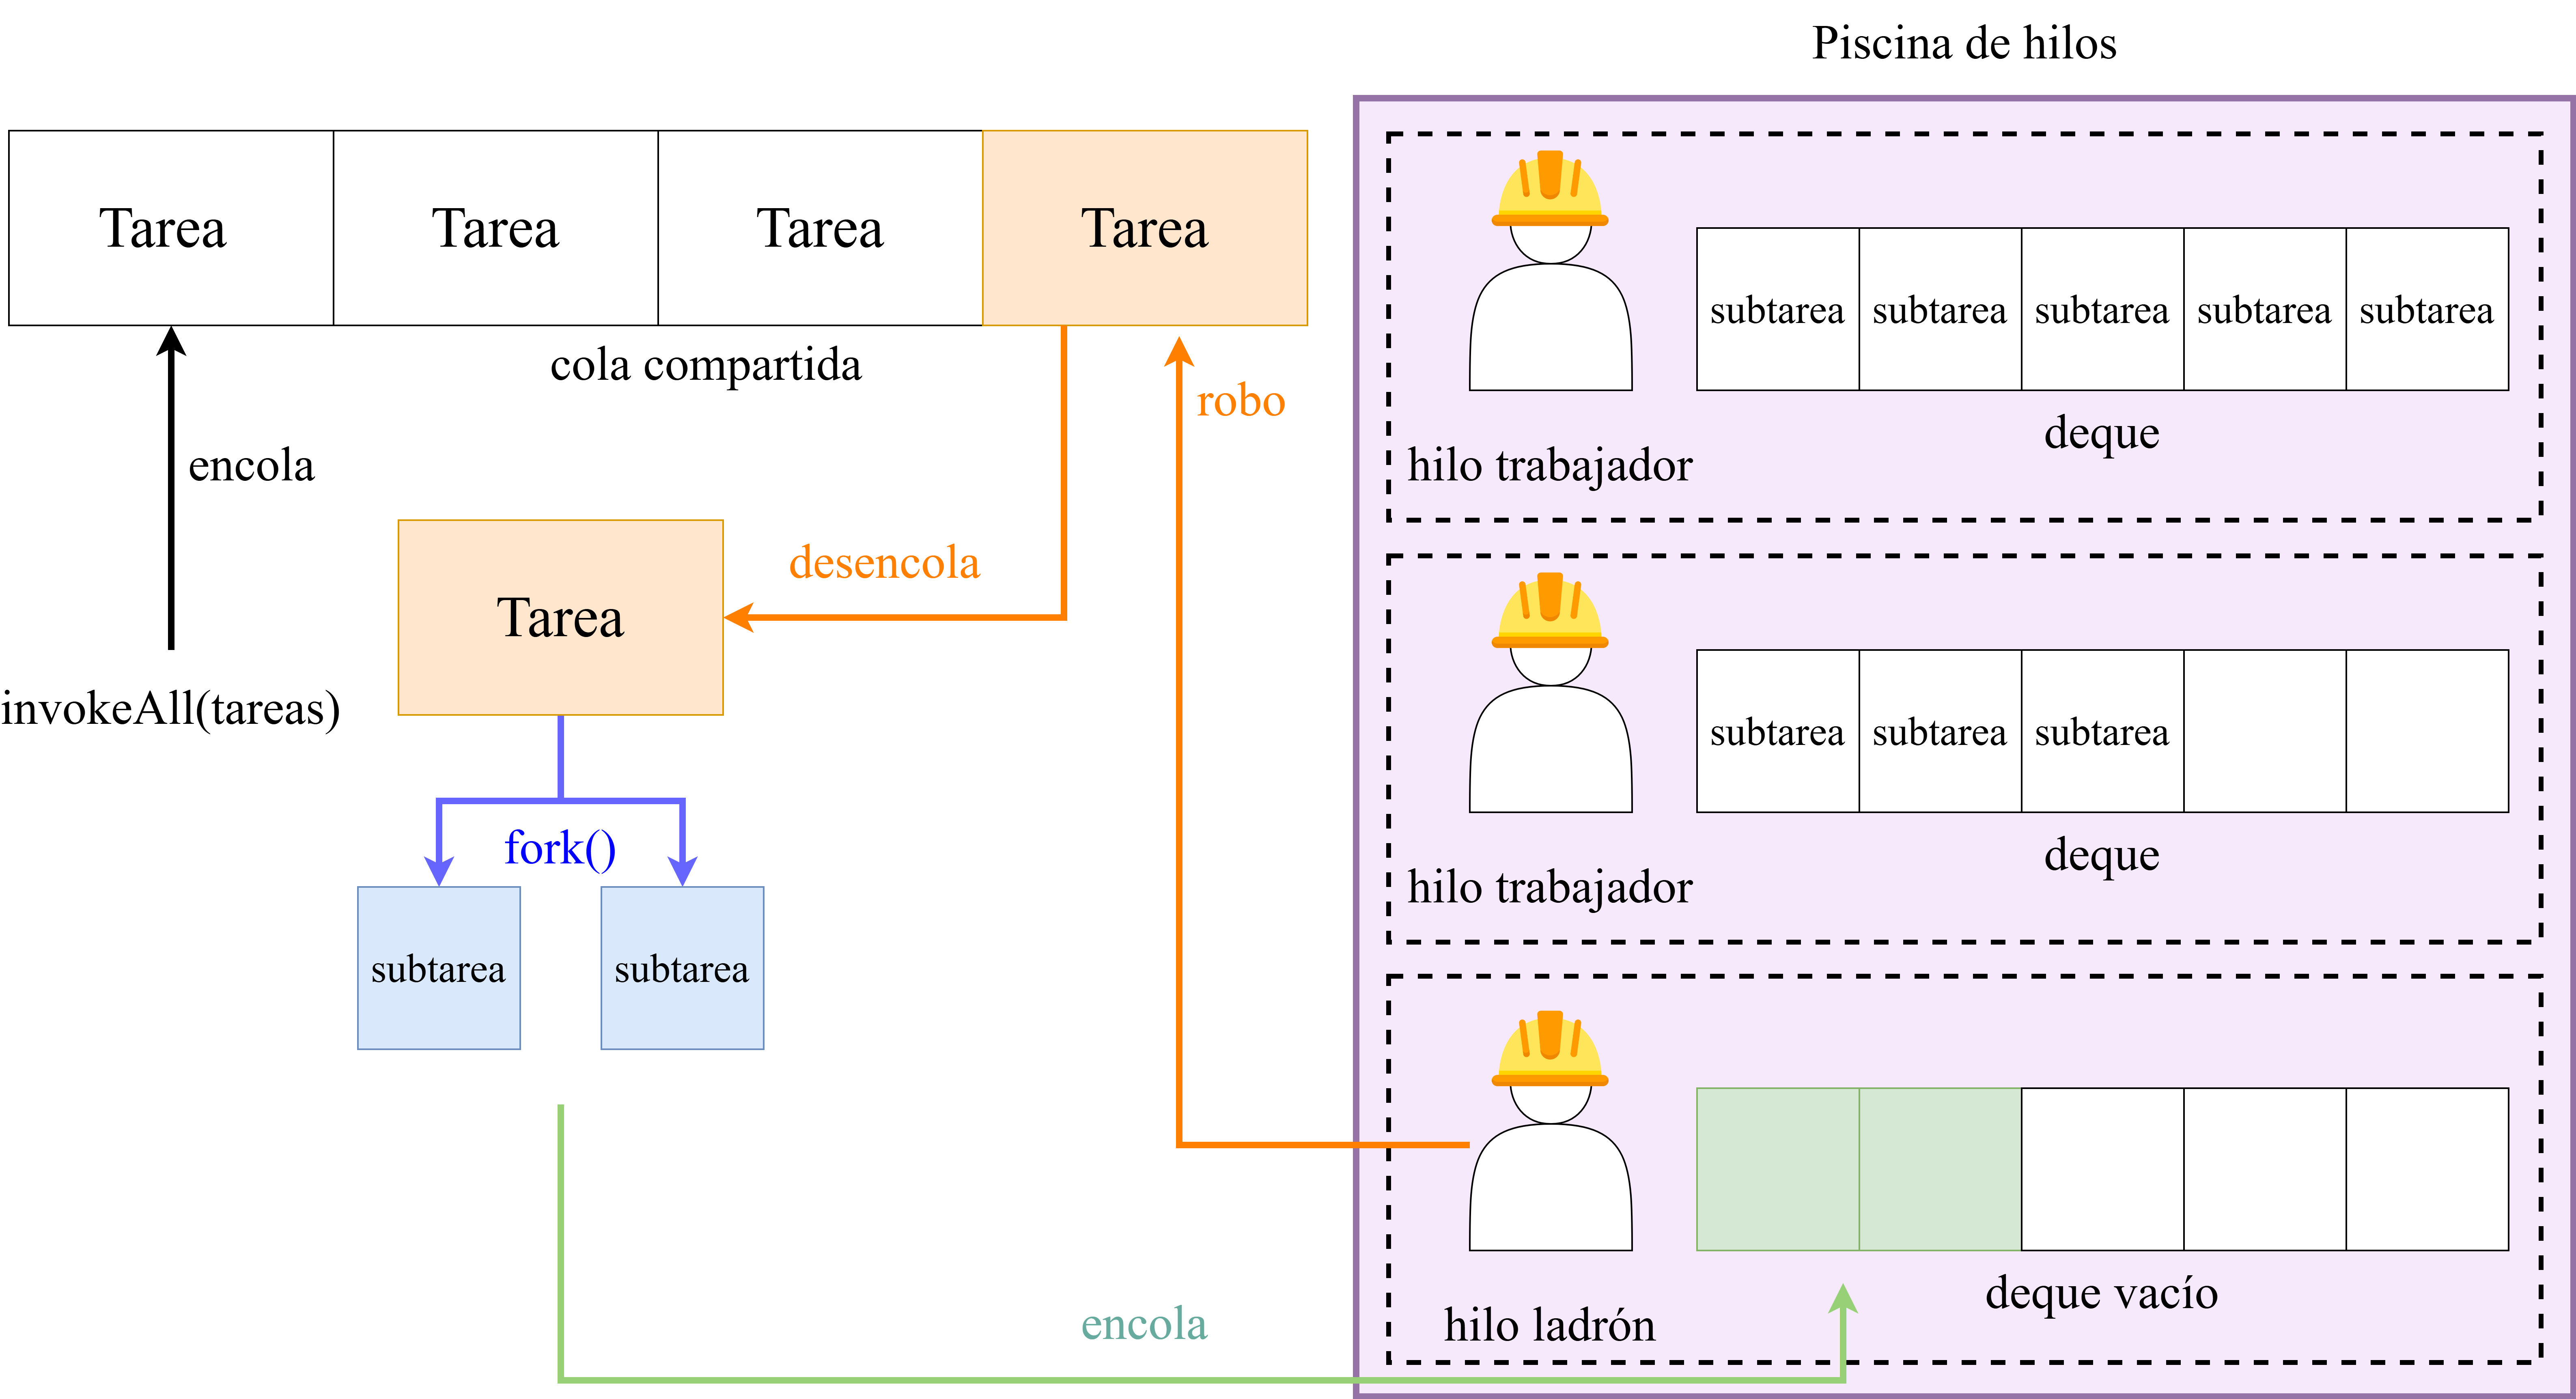
\includegraphics[width=0.75\linewidth]{Diagrames/forkJoinPool.png}
	\caption{Funcionamiento del \lstinline{ForkJoinPool}}
	\label{fig:forkJoinPool}
\end{figure}

La \lstinline{ForkJoinPool} permite crear piscinas basadas en un algoritmo de robo de trabajo (\textit{work-stealing algorithm}). \footnote{\cite{Ramgir2017-mv}} Esto significa que las tareas se acumulan en una cola compartida entre todos los hilos, pero, además, cada hilo consta de su propia cola doblemente terminada (decola). Los hilos extraen de la cola las tareas y las ejecutan, si la tarea produce subtareas estas se guardan en su decola. Puede ocurrir que la decola de un hilo se vacíe, en ese caso, el hilo desencola una tarea de la cola compartida.\footnote{\cite{kumar_2024}} La \lstinline{ForkJoinPool} es útil si el algoritmo genera muchas subtareas, ya que el uso de decolas propias reduce significativamente la cantidad de accesos a la cola compartida.\footnote[17]{} Adicionalmente, las tareas de la cola compartida serán siempre de mayor tamaño que las subtareas que generen tareas ubicadas en las decolas. Por ende, \lstinline{ForkJoinPool} es apropiada para la paralelización del \textit{Merge Sort}, en tanto que se generan subtareas que después se volverán a unir.

\begin{figure}[h]
	\begin{lstlisting}[language=java, frame=single, numbers=left]
ForkJoinPool pool = new ForkJoinPool(parallelismLevel);
MSrecursivoParalelo task = new MSrecursivoParalelo(arr, aux, left, right);
pool.invoke(task);
	\end{lstlisting}
	\caption{Inicialización de la \lstinline{ForkJoinPool}}
	\label{fig:creacionForkJoinPool}
\end{figure}

Para crear una \lstinline{ForkJoinPool} se llama a su constructor y se pasa el número de hilos trabajadores que tendrá la piscina (\lstinline{parallelismLevel}).\footnote[17]{} Después se debe pasar una tarea a la piscina que esta procesará cuando se llama al método \lstinline{.invoke()}. Existen dos tipos tareas: aquellas que no retornan ningún valor (\lstinline{RecursiveAction}) y aquellas que sí retornan (\lstinline{RecursiveTask}). Ambas subclases heredan de \lstinline{ForkJoinTask}.\footnote[17]{} En este caso, se pasa una tarea del tipo \lstinline{RecursiveAction}. (Véase la Figura \ref{fig:creacionForkJoinPool})

Concretamente, la lógica del MSRP se inscribe en una clase \lstinline{MSrecursivoParalelo} que hereda de la clase abstracta \lstinline{RecursiveAction} como se observa en la Figura \ref{fig:MSRP_RecursiveAction}. 

\begin{figure}[h]
	\begin{lstlisting}[language=java, frame=single, numbers=left]
public class MSrecursivoParaleloSinUmbral extends RecursiveAction {
	private final int[] arr, aux;
	private final int right, left;
	
	public MSrecursivoParaleloSinUmbral(int[] arr, int[] aux, int left, int right) {
		this.arr = arr;
		this.aux = aux;
		
		this.left = left;
		this.right = right;
	}
	
	@Override
	protected void compute() {	}
	
	private static void merge(int[] arr, int[] aux, int left, int mid, int right) {	}	
}    	
	\end{lstlisting}
	\caption{Esquema de la clase \lstinline{MergeSortRecursivoParalelo}}
	\label{fig:MSRP_RecursiveAction}
\end{figure}

En dicha clase el algoritmo de \textit{Merge Sort} se queda encapsulado en el método abstracto \lstinline{compute()}, como se observa en la Figura \ref{fig:MSRP_Compute}. Primero se comprueba el caso base. Después se crean dos subtareas, por ahora inactivas, para cada lado de la colección. A continuación, se pasan las subtareas a \lstinline{invokeAll()}, que las encola en la cola compartida de piscina y espera a que \lstinline{Left} y \lstinline{Right} finalicen. Finalmente, se unen las dos partes con el mismo algoritmo común \lstinline{merge()}.

\begin{figure}[h]
    \begin{lstlisting}[language=java, frame=single, numbers=left]
@Override
protected void compute() {
	if (left >= right) return;
	
	int mid = left + (right - left) / 2;
	
	final MSrecursivoParalelo Left = new MSrecursivoParalelo(arr, aux, left, mid);
	final MSrecursivoParalelo Right = new MSrecursivoParalelo(arr, aux, mid + 1, right);
	
	invokeAll(Left, Right);
	
	merge(arr, aux, left, mid, right);
}
    \end{lstlisting}
    \caption{Método \lstinline{compute()} del MSRP}
    \label{fig:MSRP_Compute}
\end{figure}

Normalmente llega un momento en que generar más subtareas torna ineficiente dado que el costo de gestión de hilos es mayor que el costo que conllevaría ejecutar las tareas de forma serial. En este caso, colecciones con baja longitud ralentizarían al MSRP. Por ende es común establecer un umbral (\textit{threshold}) a partir del cual se ejecutan las subtareas serialmente.

Se ha conducido un test piloto para determinar el umbral adecuado para esta implementación. Se han tomado 50 muestras del tiempo de ejecución para 20 longitudes de arreglo para el Merge Sort Recursivo Serial y para el Merge Sort Recursivo Paralelo, pero sin un umbral definido (como el de la Figura \ref{fig:MSRP_Compute}). En la Tabla \ref{tab:testPilotoMSRP} se comparan los promedios de las muestras obtenidas. Los tamaños de las colecciones son potencias de dos, en tanto que se intenta conseguir un árbol binario balanceado, que aprovecha mejor los recursos. Obsérvese que hasta el tamaño $2^{15}$ el algoritmo más rápido es el MSRS. Entonces se modifica el método \lstinline{compute()} para que, en caso de que la longitud del arreglo de entrada sea inferior al umbral de $2^{15}$, se ejecute la versión serial. (Figura \ref{fig:computeModificado})

\definecolor{Alto}{rgb}{0.87,0.87,0.87}
\begin{table}
	\centering
	\begin{tblr}{
			cells = {c},
			cell{1}{1} = {Alto},
			cell{1}{2} = {Alto},
			cell{1}{3} = {Alto},
			vline{1-4} = {-}{},
			hline{-} = {1-3}{},
		}
		Tamaño  & Tiempo MSRS (ms) & Tiempo MSRP sin umbral (ms) &  \\
		2       & 0,002            & 0,271                       &  \\
		4       & 0,004            & 0,325                       &  \\
		8       & 0,003            & 0,375                       &  \\
		16      & 0,003            & 0,402                       &  \\
		32      & 0,005            & 0,519                       &  \\
		64      & 0,004            & 0,751                       &  \\
		128     & 0,005            & 0,806                       &  \\
		256     & 0,013            & 0,924                       &  \\
		512     & 0,027            & 0,987                       &  \\
		1024    & 0,057            & 1,109                       &  \\
		2048    & 0,120            & 1,227                       &  \\
		4096    & 0,263            & 1,424                       &  \\
		8192    & 0,529            & 1,468                       &  \\
		16384   & 1,099            & 1,689                       &  \\
		32768   & 2,224            & 2,186                       &  \\
		65536   & 4,603            & 2,529                       &  \\
		131072  & 9,332            & 3,770                       &  \\
		262144  & 19,450           & 6,248                       &  \\
		524288  & 39,380           & 11,012                      &  \\
		1048576 & 81,661           & 25,592                      &  
	\end{tblr}
	\caption{Datos de prueba para MSRS y MSRP sin umbral} 
	\label{tab:testPilotoMSRP}
\end{table}

\begin{figure}
	\centering
	\begin{tikzpicture}
		\centering
		\begin{axis}[
			xlabel={Tamaño de la colección},
			ylabel={Tiempo (ms)},
			legend pos=north west,
			grid=major,
			width=12cm,
			height=8cm,
			xtick={1, 2, 3, 4, 5, 6, 7, 8, 9, 10, 11, 12, 13, 14, 15, 16, 17, 18, 19, 20},
			xticklabels={$$,$2^2$, $$, $2^4$, $$, $2^6$, $$, $2^8$, $$, $2^{10}$, $$, $2^{12}$, $$, $2^{14}$, $$, $2^{16}$, $$, $2^{18}$, $$, $2^{20}$}
			]
			\addplot coordinates {
				(1, 0.002) (2, 0.004) (3, 0.003) (4, 0.003) (5, 0.005) (6, 0.004) (7, 0.005) (8, 0.013) (9, 0.027) (10, 0.057) (11, 0.120) (12, 0.263) (13, 0.529) (14, 1.099) (15, 2.224) (16, 4.603) (17, 9.332) (18, 19.450) (19, 39.380) (20, 81.661)
			};
			\addlegendentry{MSRS}
			
			\addplot coordinates {
				(1, 0.271) (2, 0.325) (3, 0.375) (4, 0.402) (5, 0.519) (6, 0.751) (7, 0.806) (8, 0.924) (9, 0.987) (10, 1.109) (11, 1.227) (12, 1.424) (13, 1.468) (14, 1.689) (15, 2.186) (16, 2.529) (17, 3.770) (18, 6.248) (19, 11.012) (20, 25.592)
			};
			\addlegendentry{MSRP sin umbral}
		\end{axis}
	\end{tikzpicture}
	\caption{Datos de prueba para MSRS y MSRP sin umbral} 
	\label{fig:testPilotoMSRP}
\end{figure}

\begin{figure}[h]
	\begin{lstlisting}[language=java, frame=single, numbers=left]
protected void compute() {
	int length = (right + 1 - left);
	if (length <= THRESHOLD) {
		MSrecursivoSerial.sort(arr, aux, left, right);
	} else {
		// Ejecucion paralela
	}
}
	\end{lstlisting}
	\caption{MSRP con umbral}
	\label{fig:computeModificado}
\end{figure}

\newpage
\subsection{Merge Sort Iterativo Paralelo (MSIP)}
Para la paralelización del algoritmo iterativo se ha hecho uso de la interfaz \lstinline{ExecutorService} que proporciona Java y que proporciona un marco para gestionar y controlar la ejecución de tareas asincrónicas. A diferencia de las piscinas \lstinline{ForkJoin}, el \lstinline{ExecutorService} utiliza un algoritmo de trabajo compartido (\textit{work-sharing algorithm}). Esto implica que solo hay una cola compartida entre todos los hilos: una vez termina un hilo de ejecutar una subtarea, extrae otra de la cola. Este flujo de ejecución es apropiado para tareas independientes entre ellas.\footnote{\cite{OracleExecutorService}}.

\begin{figure}[h]
	\centering
	\begin{lstlisting}[language=java, frame=single, numbers=left]
public static void sort(int[] array, int aux[], ExecutorService executor) {
	int length = arr.length;
	List<Future<?>> futures = new ArrayList<>();
	
	for (int size = 1; size < length; size *= 2) {
		
		for (int left = 0; left < length - size; left += 2 * size) {
			int mid = left + size - 1;
			int right = Math.min(left + 2 * size - 1, length - 1);
			int finalLeft = left; //El resto son efectivamente finales
			futures.add(executor.submit(() -> merge(arr, aux, finalLeft, mid, right)));
		}
		for (Future<?> future : futures) {
			try {
				future.get();
			} catch (Exception e) {
				e.printStackTrace();
			}
		}
		futures.clear();
		
	}
	executor.shutdown();
}
	\end{lstlisting}
	
	\caption{Método \lstinline{sort()} del MSIP}
	\label{fig:MSIP_sort()}
\end{figure}

En este caso, la implementación iterativa paralela se hace en una función \lstinline{sort() } como la de la Figura \ref{fig:MSIP_sort()}. Para crear una instancia de \lstinline{ExecutorService} se usan los métodos que proporciona la clase \lstinline{Executors} de Java. Particularmente, \lstinline{.newFixedThreadPool(parallelismLevel)} crea una piscina con un número de hilos fijo determinado. 

\begin{figure}[h]
	\begin{lstlisting}[language=java, frame=single, numbers=left]
ExecutorService executorService = Executors.newFixedThreadPool(parallelismLevel);
MSiterativoParalelo.sort(arr, aux, executor);
	\end{lstlisting}
	\caption{Inicialización del \lstinline{ExecutorService}}
	\label{fig:creacionExecutorService}
\end{figure}

A continuación, para cada iteración se encola internamente en \lstinline{executor} una tarea \lstinline{merge()} mediante una expresión lambda que recibe \lstinline{executor.submit()} como argumento. Entonces un número determinado de hilos trabajadores toman las tareas de la cola interna y las ejecutan. Si todos los hilos están ocupados, la tarea esperará en la cola hasta que un hilo esté disponible. Una vez que un hilo esté disponible, tomará la tarea de la cola y la ejecutará. Cada llamada a \lstinline{merge()} implica que \lstinline{.submit()} retorne un objeto de la clase \lstinline{Future} que representa el resultado de una operación asíncrona. En este caso, se añaden los \lstinline{Future} a una lista. Finalmente se recorre la lista y para cada \lstinline{Future} se llama a \lstinline{future.get()} que obliga al hilo principal a esperar a que acaben de procesarse todas las tareas encoladas. De lo contrario, podríamos pasar al siguiente \lstinline{size} (del bucle inicial) sin asegurarse de que todas las partes están ordenadas. Una vez completado todos los bucles se llama a \lstinline{executor.shutdown()}, que espera a que, una vez terminen de ejecutarse todas las tareas encoladas anteriormente, cierra la piscina \lstinline{executor} y libera los hilos.

Al igual que en el MSRP se ha tratado de establecer un umbral, para en este caso particular cambiar a la versión iterativa serial (MSIS). Los resultados del test preliminar (Figura ) (mismo procedimiento que el anterior) arrojan que no existe tamaño de colección alguno para el cual esta implementación (MSIP) sea más rápida.

\begin{table}
	\centering
	\begin{tblr}{
			cells = {c},
			cell{1}{1} = {Alto},
			cell{1}{2} = {Alto},
			cell{1}{3} = {Alto},
			vline{1-4} = {-}{},
			hline{-} = {1-3}{},
		}
		
		Tamaño  & Tiempo MSIS (ms) & Tiempo MSIP (ms) &  \\
		2       & 0,004     & 0,240     &  \\
		4       & 0,005     & 0,432     &  \\
		8       & 0,004     & 0,649     &  \\
		16      & 0,005     & 0,645     &  \\
		32      & 0,006     & 0,504     &  \\
		64      & 0,004     & 0,504     &  \\
		128     & 0,006     & 0,605     &  \\
		256     & 0,011     & 0,685     &  \\
		512     & 0,024     & 0,663     &  \\
		1024    & 0,051     & 0,624     &  \\
		2048    & 0,111     & 0,931     &  \\
		4096    & 0,239     & 1,513     &  \\
		8192    & 0,509     & 2,686     &  \\
		16384   & 1,062     & 5,074     &  \\
		32768   & 2,197     & 9,538     &  \\
		65536   & 4,448     & 18,727    &  \\
		131072  & 8,980     & 45,305    &  \\
		262144  & 18,553    & 78,727    &  \\
		524288  & 37,924    & 173,462   &  \\
		1048576 & 78,274    & 320,937   &  
	\end{tblr}
	\caption{Datos de prueba para MSIS y MSIP sin umbral} 
	\label{tab:testPilotoMSIP}
\end{table}

\begin{figure}
	\centering
	\begin{tikzpicture}
		\begin{axis}[
			xlabel={Tamaño de la colección},
			ylabel={Tiempo (ms)},
			legend pos=north west,
			grid=major,
			width=12cm,
			height=8cm,
			xtick={1, 2, 3, 4, 5, 6, 7, 8, 9, 10, 11, 12, 13, 14, 15, 16, 17, 18, 19, 20},
			xticklabels={$$,$2^2$, $$, $2^4$, $$, $2^6$, $$, $2^8$, $$, $2^{10}$, $$, $2^{12}$, $$, $2^{14}$, $$, $2^{16}$, $$, $2^{18}$, $$, $2^{20}$}
			]
			\addplot coordinates {
				(1, 0.004) (2, 0.005) (3, 0.004) (4, 0.005) (5, 0.006) (6, 0.004) (7, 0.006) (8, 0.011) (9, 0.024) (10, 0.051) (11, 0.111) (12, 0.239) (13, 0.509) (14, 1.062) (15, 2.197) (16, 4.448) (17, 8.980) (18, 18.553) (19, 37.924) (20, 78.274)
			};
			\addlegendentry{MSIS}
			
			\addplot coordinates {
				(1, 0.240) (2, 0.432) (3, 0.649) (4, 0.645) (5, 0.504) (6, 0.504) (7, 0.605) (8, 0.685) (9, 0.663) (10, 0.624) (11, 0.931) (12, 1.513) (13, 2.686) (14, 5.074) (15, 9.538) (16, 18.727) (17, 45.305) (18, 78.727) (19, 173.462) (20, 320.937)
			};
			\addlegendentry{MSIP}
		\end{axis}
	\end{tikzpicture}
	\caption{Datos de prueba para MSIS y MSIP sin umbral} 
	\label{fig:testPilotoMSIP}
\end{figure}




\newpage
%%%%%%%%%%%%%%%METODOLOGÍA%%%%%%%%%%%%%%%%%%%%%%
%%%%%%%%%%%%%%%%%%%%%%%%%%%%%%%%%%%%%%%%%%%%%%%%

\section{Experimentación}
Para la realización de una comparación empírica de los cuatro algoritmos (MSRS, MSIS, MSRP, MSIP) se toman 50 muestras del tiempo de ejecución para $n$ tamaños de colección de entrada para cada algoritmo. Los algoritmos son ejecutados en un computador con procesador Intel(R) Core(TM) i5-11400F @ 2,60GHz y 16GB de RAM DDR4 3200MHz. En el SO de Windows 10 Pro 22H2 (x64). El IDE de ejecución es IntelliJ Idea Community Edition 2023.3.3.

\subsection{Procedimiento}

\begin{enumerate}
	\item Se generan las longitudes crecientes de las colecciones de entrada siguiendo la secuencia $n=10, 45, 100, 450, 1000... 10^8$. El máximo tamaño es $10^8$ ya que a partir de este tamaño la memoria del computador empleado es insuficiente.
	\item Para cada tamaño $n$ se genera una colección mediante la clase \lstinline{SplittableRandom} de Java, que en este caso genera colecciones de tipo \lstinline{int} con valores pseudoaleatorios extraídos de una distribución uniforme.\footnote{\cite{OracleSplittableRandom}}. Particularmente, el generador produce números del 0 al 1000 y siempre emplea la misma semilla (6180339887), por tanto, en todas las muestras la secuencia de elementos a ordenar es la misma. Esto se hace para que la variación del tiempo de ejecución a lo largo del tamaño de entrada creciente se deba a la naturaleza misma del algoritmo y no influya el estado inicial del arreglo ya que son <<idénticos>>.
	\item Para cada toma de muestra se instancia un nuevo arreglo y se copia en este el arreglo generado anteriormente; de lo contrario en la siguiente muestra se estaría ordenando un arreglo ya ordenado. Para la colección auxiliar se sigue el mismo procedimiento.
	\item El tiempo de ejecución se mide mediante la función \lstinline{System.nanoTime} que retorna el tiempo actual más preciso disponible en el sistema. El valor devuelto son los nanosegundos desde un tiempo arbitrario y provee de precisión nanosegundaria, pero no necesariamente exactitud nanosegundaria Cada ejecución se realizan entre una variable \lstinline{long startTime} y \lstinline{long endTime}. El tiempo de ejecución es la diferencia entre estas.\footnote{\cite{OracleSystem}}
	\item Después se elimina el peor y mejor tiempo de entre las 50 ejecuciones, quedando así 48.
	\item En el caso de los algoritmos paralelos se establece un mismo número de hilos para cada piscina para que la comparación sea justa. Concretamente, \lstinline{parallelism=10} ya que el computador empleado consta de 12 hilos y se reservan 2 en caso de que se ejecute algún proceso en segundo plano que los necesite. 
	\item El código de las implementaciones, el código del \textit{benchmark} y los resultados del \textit{benchmark} quedan recogidos en los Apéndices A, B y C respectivamente.
	
\end{enumerate}

\section{Discusión de resultados}

En la Tabla \ref{tab:resultadosSuperMegaDefinitivos}, se presentan los tiempos de ejecución medios en milisegundos (ms) para los cuatro algoritmos de ordenación: MSRS, MSIS, MSRP y MSIP, en función del tamaño de la colección de datos. Véase las Figura \ref{fig:tamPeq} para los tamaños pequeños (10 -- 1.000) y la Figura \ref{fig:tamMed} para los tamaños medianos (4.500 -- 450.000). Nótese que en el caso del MSIP para \(10^{8}\) no se podido mensurar el tiempo de ejecución en tanto que al ejecutar \lstinline{sort()} se ha producido una excepción \lstinline{OutOfMemoryError} indicando que Java no hay suficiente espacio en el \textit{heap} para colocar un objeto.\footnote{\cite{OracleOutOfMemoryError}} %%Hacer un mejor análisis.

\begin{table}[h]
	\centering
	\begin{tblr}{
			cells = {c},
			row{1} = {Alto},
			hlines,
			vlines,
		}
		Tamaño      & Tiempo MSRS (ms)      & Tiempo MSIS (ms)     & Tiempo MSRP (ms)     & Tiempo MSIP (ms)       \\
		10          & 0,005     & 0,009     & 0,217     & 0,842      \\
		45          & 0,008     & 0,013     & 0,227     & 0,654      \\
		100         & 0,006     & 0,009     & 0,230     & 0,629      \\
		450         & 0,024     & 0,023     & 0,265     & 0,704      \\
		1.000       & 0,054     & 0,049     & 0,330     & 0,893      \\
		4.500       & 0,275     & 0,247     & 0,530     & 1,762      \\
		10.000      & 0,636     & 0,592     & 0,936     & 3,204      \\
		45.000      & 3,067     & 2,774     & 2,137     & 13,043     \\
		100.000     & 6,855     & 6,301     & 2,765     & 33,804     \\
		450.000     & 32,441    & 30,049    & 7,527     & 134,608    \\
		1.000.000   & 74,761    & 68,275    & 14,576    & 322,416    \\
		4.500.000   & 354,405   & 332,042   & 62,903    & 1.498,327  \\
		10.000.000  & 804,113   & 749,785   & 142,320   & 3.200,823  \\
		45.000.000  & 3.825,093 & 3.570,820 & 678,702   & 15.648,251 \\
		100.000.000 & 8.534,543 & 7.889,013 & 1.535,203 & --         
	\end{tblr}
	\caption{Media de los tiempos de ejecución en ms} 
	\label{tab:resultadosSuperMegaDefinitivos}
\end{table}

El MSRS muestra un rendimiento excelente en colecciones pequeñas y medianas, con tiempos de ejecución que aumentan de manera lineal conforme crece el tamaño de la colección. A partir de $10^$

El MSIS, presenta un rendimiento muy similar al MSRS para colecciones pequeñas y medianas. Sin embargo a partir del tamaño 4500 el MSIS torna ligeramente más rápido, exceptuando el tamaño de $10^{8}$ donde el MSRS es 

Sin embargo, en colecciones grandes, el MSIS es ligeramente más rápido que el MSRS, lo que sugiere que la implementación iterativa puede ser más eficiente en ciertos casos.

\begin{figure}[H]
	\centering
	\begin{tikzpicture}
		\begin{axis}[
			xlabel={Tamaño de la colección},
			ylabel={Tiempo (ms)},
			legend pos=north west,
			grid=major,
			width=12cm,
			height=8cm,
			xtick={1, 2, 3, 4, 5, 6, 7, 8, 9, 10, 11, 12, 13, 14, 15},
			xticklabels={$10$, $$, $10^{2}$, $$, $10^{3}$, $$, $10^{4}$, $$, $10^{5}$, $$, $10^{6}$, $$, $10^{7}$, $$, $10^{8}$},
			ytickmin=0,
			ytickmax=17000,
			]
			\addplot coordinates {
				(1, 0.005) (2, 0.008) (3, 0.006) (4, 0.024) (5, 0.054) (6, 0.275) (7, 0.636) (8, 3.067) (9, 6.855) (10, 32.441) (11, 74.761) (12, 354.405) (13, 804.113) (14, 3825.093) (15, 8534.543)
			};
			\addlegendentry{MSRS}
			
			\addplot coordinates {
				(1, 0.009) (2, 0.013) (3, 0.009) (4, 0.023) (5, 0.049) (6, 0.247) (7, 0.592) (8, 2.774) (9, 6.301) (10, 30.049) (11, 68.275) (12, 332.042) (13, 749.785) (14, 3570.820) (15, 7889.013)
			};
			\addlegendentry{MSIS}
			
			\addplot coordinates {
				(1, 0.217) (2, 0.227) (3, 0.230) (4, 0.265) (5, 0.330) (6, 0.530) (7, 0.936) (8, 2.137) (9, 2.765) (10, 7.527) (11, 14.576) (12, 62.903) (13, 142.320) (14, 678.702) (15, 1535.203)
			};
			\addlegendentry{MSRP}
			
			\addplot coordinates {
				(1, 0.842) (2, 0.654) (3, 0.629) (4, 0.704) (5, 0.893) (6, 1.762) (7, 3.204) (8, 13.043) (9, 33.804) (10, 134.608) (11, 322.416) (12, 1498.327) (13, 3200.823) (14, 15648.251)
			};
			\addlegendentry{MSIP}
		\end{axis}
	\end{tikzpicture}
	\caption{Media de los tiempos de ejecución en ms} 
	\label{fig:graficoMegaFinal}
\end{figure}

\begin{figure}[H]
	\centering
	\begin{tikzpicture}
		\begin{axis}[
			xlabel={Tamaño de la colección},
			ylabel={Tiempo (ms)},
			legend pos=north west,
			grid=major,
			width=12cm,
			height=8cm,
			xtick={1, 2, 3, 4, 5},
			xticklabels={$10$, $$, $10^{2}$, $$, $10^{3}$}
			]
			\addplot coordinates {
				(1, 0.005) (2, 0.008) (3, 0.006) (4, 0.024) (5, 0.054)
			};
			\addlegendentry{MSRS}
			
			\addplot coordinates {
				(1, 0.009) (2, 0.013) (3, 0.009) (4, 0.023) (5, 0.049)
			};
			\addlegendentry{MSIS}
			
			\addplot coordinates {
				(1, 0.217) (2, 0.227) (3, 0.230) (4, 0.265) (5, 0.330)
			};
			\addlegendentry{MSRP}
			
			\addplot coordinates {
				(1, 0.842) (2, 0.654) (3, 0.629) (4, 0.704) (5, 0.893)
			};
			\addlegendentry{MSIP}
		\end{axis}
	\end{tikzpicture}
	\caption{Media de los tiempos de ejecución en ms para tamaños pequeños} 
	\label{fig:tamPeq}
\end{figure}

\begin{figure}[H]
	\centering
	\begin{tikzpicture}
		\begin{axis}[
			xlabel={Tamaño de la colección},
			ylabel={Tiempo (ms)},
			legend pos=north west,
			grid=major,
			width=12cm,
			height=8cm,
			xtick={1, 2, 3, 4, 5},
			xticklabels={$10$, $$, $10^{2}$, $$, $10^{3}$, $$, $10^{4}$, $$, $10^{5}$, $$}
			]
			\addplot coordinates {
				(1, 0.005) (2, 0.008) (3, 0.006) (4, 0.024) (5, 0.054) (6, 0.275) (7, 0.636) (8, 3.067) (9, 6.855) (10, 32.441)
			};
			\addlegendentry{MSRS}
			
			\addplot coordinates {
				(1, 0.009) (2, 0.013) (3, 0.009) (4, 0.023) (5, 0.049) (6, 0.247) (7, 0.592) (8, 2.774) (9, 6.301) (10, 30.049)
			};
			\addlegendentry{MSIS}
			
			\addplot coordinates {
				(1, 0.217) (2, 0.227) (3, 0.230) (4, 0.265) (5, 0.330) (6, 0.530) (7, 0.936) (8, 2.137) (9, 2.765) (10, 7.527)
			};
			\addlegendentry{MSRP}
			
			\addplot coordinates {
				(1, 0.842) (2, 0.654) (3, 0.629) (4, 0.704) (5, 0.893) (6, 1.762) (7, 3.204) (8, 13.043) (9, 33.804) (10, 134.608)
			};
			\addlegendentry{MSIP}
		\end{axis}
	\end{tikzpicture}
	\caption{Media de los tiempos de ejecución en ms para tamaños medianos} 
	\label{fig:tamMed}
\end{figure}

\subsection{Comparación}
\subsection{Conclusión}

\section{Bibliografía}
\bibliography{bibliografia}
\section{Anexo}

\end{document}